%
\documentclass[12pt,notitlepage]{article}
\usepackage{amssymb}
\usepackage{amsmath}
\usepackage{graphicx}
\usepackage{epstopdf}
\usepackage{pdflscape}
\usepackage[pdftex,dvipsnames]{xcolor}
\setlength{\marginparwidth}{2cm}
\usepackage[colorinlistoftodos,prependcaption,textsize=small]{todonotes}
\usepackage{xargs}
\usepackage{tabularx}
\usepackage{longtable}
\usepackage{arydshln}
\usepackage{array}
\usepackage{dsfont}
\usepackage{float}
\usepackage{booktabs}
\usepackage{tikz}
\usepackage{marvosym}
\usepackage{multirow}
\usepackage{pdflscape}
\usepackage[hyphens]{url}
\usepackage{setspace}
\usepackage{epigraph}
\usepackage{bm}
\usepackage{textcomp}
\usepackage{diagbox}
\usepackage{bbm}
\usepackage{verbatim}
\usepackage[framemethod=tikz]{mdframed}
\usepackage{subcaption}
\captionsetup[sub]{subrefformat=parens}
\DeclareCaptionLabelFormat{subpanel}{Panel~(#2):}
\captionsetup[sub]{labelformat=subpanel, labelsep=space}

\usepackage{caption}
\usepackage{lipsum}
\usepackage{mathtools}
\usepackage{scalerel}
\usepackage{stackengine}
\usepackage{amsthm}
\usepackage{epsfig}
\usepackage[
backend=biber,
authordate, 
]{biblatex-chicago}

\usepackage[colorlinks,allcolors=blue]{hyperref}
\usepackage[shortlabels]{enumitem}
\usepackage{subfiles} % Best loaded last in the preamble


\setlength{\epigraphrule}{0pt}
\renewcommand{\baselinestretch}{1.25}

\setcounter{MaxMatrixCols}{10}

\newcolumntype{L}[1]{>{\raggedright\let\newline\\arraybackslash\hspace{0pt}}m{#1}}
\newcolumntype{C}[1]{>{\centering\let\newline\\arraybackslash\hspace{0pt}}m{#1}}
\newcolumntype{R}[1]{>{\raggedleft\let\newline\\arraybackslash\hspace{0pt}}m{#1}}



\newcommand{\I}{\mathbb{I}}
\newcommand{\E}{\mathbb{E}}
\newcommand{\Ll}{\mathrm{L}}
\newcommand{\R}{\mathbb{R}}
\renewcommand{\L}{\mathbb{L}}
\newcommand{\Var}{\mathrm{Var}}
\newcommand{\Cov}{\mathrm{Cov}}
\newcommand{\Corr}{\mathrm{Corr}}
\newcommand{\Prob}{\mathbb{P}}
\newcommand{\supp}{\mathrm{supp}}
\newcommand{\notimplies}{\mathrel{{\ooalign{\hidewidth$\not\phantom{=}$\hidewidth\cr$\implies$}}}}
\newcommand{\var}{\mathrm{var}}
\newcommand{\Bias}{\mathrm{Bias}}
\newcommand{\cov}{\mathrm{cov}}
\newcommand{\corr}{\mathrm{corr}}
\newcommand{\MSE}{\mathrm{MSE}}
\let\OldTodo\todo

\RenewDocumentCommand{\todo}{O{} m}{\OldTodo[#1]{\textbf{TODO}: #2}}
\newcommandx{\thiswillnotshow}[2][1=]{\OldTodo[disable,#1]{#2}}
\newcommandx{\askjesse}[2][1=]{\OldTodo[linecolor=Plum,backgroundcolor=Plum!25,bordercolor=Plum,#1]{\textbf{{Ask Jesse:}} #2}}
\newcommandx{\longterm}[2][1=]{\OldTodo[linecolor=Blue,backgroundcolor=Blue!25,bordercolor=Blue,#1]{\textbf{{Long-term:}} #2}}
\newcommandx{\donow}[2][1=]{\OldTodo[linecolor=Green,backgroundcolor=Green!25,bordercolor=Green,#1]{\textbf{{Do Now:}} #2}}


\topmargin=-1.5cm \textheight=23cm \oddsidemargin=0.5cm
\evensidemargin=0.5cm \textwidth=15.5cm

\newtheorem{theorem1}{Special Theorem}

\newtheorem{ass}{Assumption}
\newtheorem{definit}{Definition}
\newtheorem{prop}{Proposition}
\newtheorem{thm}{Theorem}
\newtheorem{lem}{Lemma}
\newtheorem{conj}{Conjecture}
\newtheorem{cor}{Corollary}
\newtheorem{rem}{Remark}

\renewcommand{\thesubsection}{\arabic{section}.\arabic{subsection}}
\renewcommand{\thesubsubsection}{\arabic{section}.\arabic{subsection}.\arabic{subsubsection}}

\newcommand\dapprox{\stackrel{\mathclap{\tiny \mbox{d}}}{\approx}}
\newcommand\papprox{\stackrel{\mathclap{\tiny \mbox{p}}}{\approx}}
\newcommand\pconverge{\stackrel{\mathclap{\tiny \mbox{p}}}{\to}}
\newcommand\dconverge{\stackrel{\mathclap{\tiny \mbox{d}}}{\to}}

\addbibresource{source/paper/references.bib}


\newcommand\independent{\protect\mathpalette{\protect\independenT}{\perp}}
\def\independenT#1#2{\mathrel{\rlap{$#1#2$}\mkern2mu{#1#2}}}

\onehalfspacing
\newtheorem{theorem}{Theorem}
\newtheorem{corollary}[theorem]{Corollary}
\newtheorem{proposition}{Proposition}

\newtheorem{hyp}{Hypothesis}
\newtheorem{subhyp}{Hypothesis}[hyp]
\renewcommand{\thesubhyp}{\thehyp\alph{subhyp}}

\newcommand{\red}[1]{{\color{red} #1}}
\newcommand{\blue}[1]{{\color{blue} #1}}


% required by modelsummary
\usepackage{tabularray}
\usepackage{float}
\usepackage{graphicx}
\usepackage{codehigh}
\usepackage[normalem]{ulem}
\UseTblrLibrary{booktabs}
\UseTblrLibrary{siunitx}
\newcommand{\tinytableTabularrayUnderline}[1]{\underline{#1}}
\newcommand{\tinytableTabularrayStrikeout}[1]{\sout{#1}}
\NewTableCommand{\tinytableDefineColor}[3]{\definecolor{#1}{#2}{#3}}


\begin{document}

\begin{titlepage}
\title{Organizational Resilience: Evidence from Open Source Software}
\author{Christopher Liao\thanks{I am indebted to Jesse Shapiro and Ali Hortaçsu for their support and guidance. I also thank Noah Sobel-Lewin, Krishna Dasari, Anjali Pullabhotla, Jeff Gortmaker, Ruru Hoong, Ruby Zhang, Matthew Lee Chen, Emanuel Scherz and members of the Harvard Predoc Workshop and Jesse Morgan Shapiro Lab for helpful comments and suggestions. This work builds on my undergraduate thesis, which benefited from discussions with Luis Garicano, Jordan Rosenthal-Kay, James Traina, Victor Lima, Kotaro Yoshida and the UChicago Economics Honors Workshop.}}
\date{\today}
\maketitle

\iffalse
\begin{abstract}
\noindent Placeholder\\
\vspace{0in}\\
\noindent\textbf{Keywords:} key1, key2, key3\\

\bigskip
\end{abstract}
\fi

\setcounter{page}{0}
\thispagestyle{empty}
\end{titlepage}
\pagebreak \newpage

\section{Introduction} \label{sec:intro}
% \textbf{Paragraphs 1-2: Motivation. After reading these paragraphs a reader in any field of economics should believe that if you answer your research question your paper will make an important contribution.}

All organizations will face challenges. Some crumble under pressure. Others are able to weather the storm, bouncing not just back, but forward. 
These are resilient organizations. Building a resilient organization that successfully navigate disruptions to environment is a topic of great interest. 
Witness, for instance, the myriad of organizational resilience insights produced by McKinsey \& Company (\cite{maor_building_2022}, \cite{maor_foster_2023}, \cite{kristensen_building_2025}), academic papers in fields from business research (\cite{duchek_organizational_2020}) to health policy (\cite{barasa_what_2018}) or teaching cases in industries such as journalism (\cite{dutton_heart_2010}), cloud technology services (\cite{tang_business_2025}) and healthcare (\cite{atkinson_organizational_2023}). 
But what organizational practices actually contribute to organizational resilience, enabling organizations ``to maintain or restore an acceptable level of functioning despite perturbations or failures.'' (\cite{robert_organizational_2009})

A wide variety of organizational practices have been found to bolster organizational resilience, from investing in talent (\cite{maor_building_2022}) and promoting positive communication (\cite{luthans_psychological_2006}) to establishing shared knowledge via resource or knowledge redundancy (\cite{sheffi_supply_2005}, \cite{rashid_systematic_2019}) and establishing routine s(\cite{suarez_building_2020}). 
Yet, despite the prevalence of research on organizational resilience and the high levels among the broader business community, there does not exist an systematic empirical analysis of what factors contribute to organizational resilience. 
Addressing this gap is important because it will help us understand whether existing beliefs about organizational resilience based off case studies, surveys or personal experience are generalizable.
% on redundancy Linnenluecke, Martina K., and Andrew Griffiths. 2010. Beyond adaptation: resilience for business in light of climate change and weather extremes. Business and Society 49: 477–511.

% \textbf{Paragraphs 3-4: Challenges. These paragraphs explain why your research question has not already been answered, i.e., what are the central challenges a researcher must tackle to answer this question.}

A systematic empirical analysis of what organizational practices contribute to organizational resilience question requires addressing two challenges.
The first challenge is that measurement of organizational practices is difficult. 
The most detailed measures of organizational practices are derived from the actions of individual members. 
Yet member-level data—such as how much they work, what tasks they undertake, and with whom they work with—is often unavailable to researchers. 
Even studies that draw on high-quality administrative records of individuals and firms or comprehensive surveys of management practices, are unable to speak to the day-to-day activities of members and how these activities contribute to or reflect broader organizational practices (\cite{bloom_management_2012}, \cite{jaravel_team-specific_2018}, \cite{jager_how_2022}). 

The second challenge is developing a general and convincing measure of organizational resilience. 
Organizational resilience can only be assessed by examining how an organization responds to disruptions. 
A systematic comparison requires assessing organizations along comparable outcomes and in relation to the same type of disruption. 
This ensures that differences in resilience reflect differences in organizational practices rather than differences in the nature of the disruption. 
Identifying a plausibly exogenous disruption is also critical to ensure that variation in organizational outcomes can be attributed to differences in resilience rather than to unobserved trends.

In this paper, I study organizational resilience in open source software (OSS) organizations, where member-level data on activities is available. 
I use the departures of key organizational members as the window into understanding what organizational practices contribute to organizational resilience. 
I measure organizational resilience by assessing how the open source software's development activity, release frequency, and usage are affected following a key member’s departure.
I then investigate how four types of organizational practices contribute to organizational resilience post-departure: practices that build knowledge redundancy, invest in member human capital, establish organizational routines, and reflect organizational adaptivity.  
These practices are selected based off their relevance in literature reviews on organizational resilience research

% \textbf{Paragraph 5: This Paper. This paragraph states in a nutshell what the paper accomplishes and how. }


% \longterm[inline]{Paragraphs 6-7: Model. Summarize the key formal assumptions you will maintain in your analysis.

% \textbf{Paragraphs 8-9: Data. Explain where you obtain your data and how you measure the concepts that are central to your study}

OSS refers to software that is freely available for use and modification and is considered a public good. 
OSS is pervasive - a recent report found that 97\% of all software included OSS code (\cite{fred_bals_six_2025}). 
Prominent examples of OSS organizations include the operating system Linux, the operating system of choice for 96.4\% of the top one million web servers (\cite{w3cook_os_2015})\footnote{Ubuntu, CentOS, Debian, Fedora, SUSE and Redhat are all Linux-based} and the machine learning framework PyTorch, which is used by 63\% of all organizations training machine learning models (\cite{lawson_shaping_2024}). 
Data from the GitHub Archive (\cite{github_archive_github_2025}) expose the contributions and communications of members within OSS organizations, enabling me to characterize organizational practices. 

To measure knowledge redundancy, I assess the extent of collaboration within organizations and the degree to which members act as specialists or generalists, based on the range of tasks they perform. To measure investment in human capital, I evaluate the timeliness, frequency, and positivity of feedback provided to members, the cohesiveness of the organization's social structure, and the frequency of internal advancement. To measure organizational routines, I examine the extent to which organizations formalize processes for problem description, problem solving, approving solutions, and problem assignment. Finally, to assess organizational adaptivity, I analyze how organizations reallocate members in response to delays or lags.

% \textbf{Paragraphs 10-11: Methods. Explain how you take your model to the data and how you overcome the challenges you raised in paragraphs 3-4.}

Identifying the causal effect of departures is necessary for my measure of resilience, but challenging because departures can occur for personal reasons unobservable to the researcher, such as personal dissatisfaction with the organization (\cite{hannon_retaining_2008}, \cite{yu_empirical_2012}), which may itself be driven by underlying trends in organizational outcomes. 
To identify a set of important departures that are plausibly exogenous to underlying trends in organizational outcomes, I use the data on OSS organizations to isolate abrupt departures. 
Abrupt departures occur when a member ceases all contributions to the organization immediately after several periods of high activity. 
Survey evidence shows that abrupt departures by important members tend to be motivated by shocks to a member's time budget unrelated to underlying organization trends, such as job changes or major life events (\cite{miller_why_2019}). 
In contrast, other forms of departures tend to be associated with unobservable organizational factors, such as disengagement with the organization's social community or personal dissatisfaction with leadership (\cite{yu_empirical_2012}, \cite{constantinou_empirical_2017}, \cite{miller_why_2019}).

I estimate the empirical effect of important departures on organization outcomes using an event study design.
The treatment date is the time period immediately following an important departure. 
I restrict the sample to organizations that only ever experience a single important departure, so that the treatment is binary, irreversible and absorbing. 
My primary estimation method is \cite{callaway_difference--differences_2021}, which allows me to estimate dynamic treatment effects robust to heterogeneity in treatment timing using the set of ``not-yet-treated'' organizations as controls. 

To analyze how organizational practices affect organizational resilience, I subset organizations based off their pre-departure organizational practices and estimate separate event studies for each subset. Since differences in pre-departure organizational practices may differ across organizations due to endogenous factors, I leverage the microdata on OSS organizations and members to show the direct mechanisms by which different organizational practices affect organizational resilience. 

% \textbf{Paragraphs 12-13: Findings. Describe the key findings. Make sure they connect clearly to the motivation in paragraphs 1-2.}
% \todo[inline]{It would be nice to place a number on "impacts" caused by departure (what's the headline number?)}

\todo[inline]{Results to come}

% I also want a robustness for departures (that are vs. aren't abrupt) using that departure filtering event study graph

% \textbf{Paragraphs 14-15: Literature. Lay out the two main ways your paper contributes to the literature. Each paragraph should center around one contribution and should explain precisely how your paper differs from the most closely related recent work.}

While a large literature in economics has examined how organizational structure influences organizational outcomes (\cite{bloom_measuring_2007}, \cite{brynjolfsson_complementarity_2012}, \cite{ichniowski_insider_2012}), research on organizational resilience has primarily emerged from the management literature (\cite{annarelli_strategic_2016}, \cite{hillmann_organizational_2021}). 
However, empirical work on organizational resilience has largely consisted of case studies and surveys (see Table 2 of \cite{annarelli_strategic_2016}) or contributions to the measurement of organizational resilience (\cite{hillmann_organizational_2021}). 
A large body of work in economics has also examined the impact of plausibly exogenous departures on labor demand (\cite{jager_how_2022}) and collaborations among inventors (\cite{agrawal_how_2008}, \cite{jaravel_team-specific_2018}, \cite{azoulay_does_2019}), academics (\cite{waldinger_quality_2010},\cite{oettl_reconceptualizing_2012}), scientists (\cite{khanna_aftermath_2021}) and doctors (\cite{chen_team-specific_2021}). 

The most closely related work is \cite{jaravel_team-specific_2018}, who leverage plausibly exogenous disruptions to a team (via the premature death of an inventor) to understand the impact of past collaboration. 
However, while \cite{jaravel_team-specific_2018} examines why some co-inventors are worse off following the premature death of a collaborator, I investigate why some organizations may be better off following a member’s departure, with the aim of identifying practices that enhance resilience implementable by organizations. 
I am able to pursue this question due to the granularity of my organizational data, a feature largely absent from data used by related work. I am also evaluating several organizational practices adopted by the organization, as opposed to just collaboration among members. 

This work contributes also contributes to the economics literature on open source software (OSS) and organizational structure. 
Past work has explored how open source software organizations are organized (\cite{mockus_two_2002}, \cite{crowston_coordination_2005}, \cite{den_besten_allocation_2008}) and the factors that determine organization success (\cite{mustonen_copyleft--economics_2003}, \cite{fershtman_open_2007}, \cite{comino_planning_2007}, \cite{belenzon_motivation_2008}, \cite{giuri_skills_2010}). 
However, work related specifically to what makes organizations resilient post-departure is a more active research topic in the information systems and software engineering literature. 
\cite{rashid_systematic_2019} provides an detailed overview of that literature. 
There has been extensive conceptual, survey and case study work  on the prevalence and ways OSS organizations can mitigate departures (\cite{robles_evolution_2005}, \cite{hannon_retaining_2008}, \cite{westlund_retaining_2008}, \cite{xu_volunteers_2010}, \cite{yu_empirical_2012}, \cite{miller_why_2019}) and how members can engage in ``knowledge sharing" behaviors (\cite{von_krogh_community_2003}, \cite{rashid_exploring_2017}) within an OSS organization. 
Prior empirical work has sough to quantify the impact of departures through metrics characterizing potential damage to the codebase (\cite{izquierdo-cortazar_using_2009}, \cite{rigby_quantifying_2016}, \cite{nassif_revisiting_2017}). 

\cite{rigby_quantifying_2016}, which is most closely related to this paper, finds that the presence of “successors” who worked on tasks similar to the departed member can mitigate the repercussions of departures, though there are important differences. 
First, I focus on a variety of organizational practices, as opposed to just one. 
Second, whereas \cite{rigby_quantifying_2016} analyzes all departures from just 5 organizations, my analysis includes many more projects. 
Finally, while \cite{rigby_quantifying_2016} considers hypothetical impacts based on potential codebase damage and possible mitigation through a successor, I quantify using realized outcomes measuring organizational resilience, the actual impact of organizational practices. 

\newpage
\section{Data} \label{sec:data}
\subsection{Data sample}

I am interested in OSS organizations that develop widely used Python libraries - defined as libraries with at least 1000 monthly downloads each month from September 2018 to July 2023. I focus on the subset of organizations whose development data is publicly available on GitHub. 

The unit of observation is an open source software organization. In Panel~\subref{fig:dask-home} of Figure~\ref{fig:dask-screenshots}, I show an example homepage for the Github organization \textbf{dask/dask}. Each open source software organization has members who work on problems. Conceptually, a problem consist of at least one of two components: discussion and solution evaluation. To initiate discussion of a problem, a member opens an issue, and discussion occurs in the issue thread. Panel~\subref{fig:dask-issue} of Figure~\ref{fig:dask-screenshots} depicts an example issue thread. If a solution is required for a particular problem, members will make code changes. The solver can open a pull request (PR) that is linked to a solution and requests others to review their solution prior to incorporating it into the software. Any general subsequent discussion that occurs regarding the pull request occurs in the pull request thread, and any discussion about specific code changes (with references to the code) occur in the pull request thread.\footnote{There are two exceptions. First, sometimes these code changes are implemented without approval. Second, sometimes pull requests are opened without a prior discussion} Solutions consist of changes to the software's codebase. Each change is called a commit. I define an OSS organization’s activity within a time period as all activity within a six-month interval—either January through June or July through December of the relevant calendar year and my period of observation spans from 2015 to the first half of 2023. Panel~\subref{fig:organization-summary-stats} provides further summary statistics on organization activity and members. All aforementioned data on development activity are obtained from the GitHub Archive (\cite{github_archive_github_2025}), via Google BigQuery.

\donow[inline]{
Provide insight into what a organization is like with a table and add other summary stats that may be interesting as I read the paper (don't delete this)
}

\subsection{Departures, Collaboration and Important members}
\subsubsection{Defining member Departures}
I am interested in the departure effects of members who worked extensively on code development, defined as those with contributions (measured in commit counts) above the 75th percentile in each period for at least 3 consecutive periods. From this subset, I classify a member as “departed” if, after ranking above the 75th percentile of commits for at least three consecutive periods, their activity across all areas (commits, discussion participation, etc) ceases in the immediately following period and remains at that state for all future observable periods. I subset to organizations that only experience one departure to simplify the identification of treatment effects. Finally, I subset to only include organizations with at least 2 important members (defined in Section~\ref{sec:collab_imp_contr}) and at least 5 pull requests opened in each of the periods prior to departure. This leaves me with 80 departed members, and hence 80 organizations. Panel~\subref{fig:departed-summary-stats} of Figure~\ref{fig:summary-stats} displays the number of members left after each successful filtering. 

\todo[inline]{Use autofills for 80 + summary stats table}

\subsubsection{Defining Collaboration and Important members} \label{sec:collab_imp_contr}

I focus exclusively on collaboration between the departing member and other important members for three reasons related to the OSS community. First, extensive interactions with unimportant members are uncommon because unimportant members typically aim only to have their own solutions adopted, rather than to engage with the broader community (\cite{hippel_open_2003}). Second, collaborations in which a non-key member does engage with a key member are largely procedural, as important members must approve pull requests opened by unimportant members, so variation offers little insight into voluntary collaborative behavior. Finally, behavior among important members is most interesting in OSS organizations because at important members are vastly more influential in shaping organization outcomes and code changes (\cite{crowston_core_2006}). 

To operationalize collaboration with the departed, I must first specify what constitutes an “important member.” The concept that there is a wide gulf of importance between certain members and others is accepted in the literature. Prior case studies of the OSS community (\cite{cox_cathedrals_1998}, \cite{mockus_two_2002}, \cite{gacek_many_2004}) have suggested that the structure of OSS organizations is akin to a hierarchy.

One natural criterion to evaluate a member's importance is to base it off their involvement in organizational discussions. To operationalize this, I construct an undirected social network characterizing discussions in each time period (following the procedure in \cite{crowston_hierarchy_2006}). Nodes represent members and edge weights record the number of exchanges in issue and pull request threads. If one member’s comment follows another’s within the same thread, I treat that as one exchange. For example, the conversation depicted in Panel~\subref{fig:dask-issue} of Figure~\ref{fig:dask-screenshots} would represent two exchanges between the users engaging in the conversation. A member is deemed important in period $t$ if, during any of the three most recent periods ($t-2, t-1$ or $t$) they are active and satisfy at least one of the following two criteria:
\begin{enumerate}
    \item Among all members active in period $t$, the number of unique peers they have exchanged messages (termed as their network degree) has a $z$‐score exceeding 1.5 or ranks highest among all members, OR
    \item they are the focal departed member under study. 
\end{enumerate} 

\subsection{Defining Collaboration} \label{sec:defining_collab}
A given organization $i$ in time period $t$ faces problems $P_{i,t} = \{p_{i,t}^1, \cdots, p_{i,t}^{N_{i,t}} \}$ where $N_{i,t}$ is the number of problems faced by organization $i$ in time period $t$. 
\begin{itemize}
\item Let $C_{i,t}$ denote the set of all members to organization $i$ in time $t$ decomposed into the set of important and unimportant members: $C_{i,t} = C_{i,t}^{imp} \cup C_{i,t}^{other}$ 
\item For each problem $p_{i,t}^k$ you have a set of collaborators $C_{i,t}^{k} \subseteq C_{i,t}^{imp} $ that consists of important ($C_{i,t}^{k, imp} = C_{i,t}^{k} \cap C_{i,t}^{imp}$) and unimportant collaborators ($C_{i,t}^{k, other} = C_{i,t}^{k} \cap C_{i,t}^{other}$)
\end{itemize}
Collaboration occurs in a problem when 2 or more important members are both involved. Hence, overall collaborativeness is deined as as 
\begin{equation}
\mathrm{OverallCollab}_{i,t} = \frac{1}{N_{i,t}}\sum_{k=1}^{N_{i,t}}\mathbf{1}\bigl\{|C_{i,t}^{k,imp}|\ge2\bigr\}
\end{equation}
The collaboration score has a nice decomposition. Let $d$ denote the departed member. I can then define $P_{i,t}^d = \{p_{i,t}^{k} \mid d \in C_{i,t}^k, 1 \leq k \leq N_{i,t} \}$ as the set of problems where the departed member $d$ is involved and $N_{i, t}^d = |P_{i,t}^d|$ as the number of problems where the departed member is involved. 
I can describe the overall collaborativeness as a function of collaborativeness metrics that involve and totally exclude the departed member. 
Define 
\begin{align*}
 \mathrm{DepartedCollab}_{i,t} &= \frac{1}{N_{i,t}^d} \sum_{k \in P_{i,t}^d} \mathbf{1}\bigl\{|C_{i,t}^{k,\mathrm{key}}|\ge2\bigr\} \\
 \mathrm{OtherCollab}_{i,t} &= \frac{1}{N-N_{i,t}^{d}} \sum_{k \notin P_{i,t}^d} \mathbf{1}\bigl\{|C_{i,t}^{k,\mathrm{key}}|\ge2\bigr\}
\end{align*}
then I can rewrite $\mathrm{OverallCollab_{i,t}}$ as the following
\begin{align*}
\mathrm{OverallCollab}_{i,t} &= \frac{N_{i,t}^d}{N_{i,t}} \frac{1}{N_{i,t}^d} \sum_{k \in P_{i,t}^d} \mathbf{1}\bigl\{|C_{i,t}^{k,\mathrm{key}}|\ge2\bigr\} + \frac{N_{i,t}-N_{i,t}^{d}}{N_{i,t}} \frac{1}{N_{i,t}-N_{i,t}^{d}} \sum_{k \notin P_{i,t}^d} \mathbf{1}\bigl\{|C_{i,t}^{k,\mathrm{key}}|\ge2\bigr\} \\
&= \frac{N_{i,t}^d}{N_{i,t}}\mathrm{DepartedCollab}_{i,t} + \frac{N_{i,t}-N_{i,t}^{d}}{N_{i,t}} \mathrm{OtherCollab}_{i,t}
\end{align*}
Henceforth, most collaboration-related analyses will focus on $\mathrm{DepartedCollab}_{i,t}$. 

\section{Methods} \label{sec:method}
\subsection{Estimating the impact of departures} \label{sec:main_method}
My primary outcome of interest $y_{i,t}$ is the number of pull requests opened by organization $i$ in time period $t$. I focus on pull requests because they are the most direct measure of production effort that organizations are engaging in. I transform the outcome into a z-score to enable cross-organization comparisons under one unit - standard deviations - which accounts for underlying cross-organization differences in the number of pull requests opened. To avoid contaminating treatment effect estimation with the outcome, I standardize based on the pre-treatment mean and standard deviation, calculated using the 4 periods prior to treatment.

Denote by $G_i$ the first period where organization $i$'s departed member is no longer part of the organization. Accordingly, organization $i$'s treatment indicator at time $t$ is defined as
$$
D_{i,t} = \mathbf{1}\{t \ge G_i\}.
$$

Define a cohort $g$ as organizations with the same treatment date $g = G_i$. For all $t \geq g$, I define the group‐time average treatment effect as 
\begin{align*} \label{eq:group_time}
    \mathrm{ATT}(g,t) = \mathbb{E}\bigl [ y_{i,t}(1)-y_{i,t}(0)\mid G_i = g \bigr ].
\end{align*}
Let $k = t - g$. Our primary estimate of interest, the average effect \(k\) periods after departure is
\begin{align*} 
\mathrm{ATT}(k) =
\mathbb{E}\bigl[y_{i,G_i+k}(1)-y_{i,G_i+k}(0)\bigr] = 
\sum_{g} \Pr\!\bigl(G_i = g \mid G_i + k \le T\bigr)\,\mathrm{ATT}\bigl(g,\,g+k\bigr).
\end{align*} 

My estimation does not involve covariates so I can ignore the overlap assumption from \cite{callaway_difference--differences_2021}. Treatment is irreversible, by definition of $D_{i,t}$ and I assume that $\{Y_{i,1},\dots,Y_{i,T},D_{i,1},\dots,D_{i,T}\}_{i=1}^n$ are independent and identically distributed. As such, identification of $\mathrm{ATT}(g,t)$ (and hence $\mathrm{ATT}(k)$) requires the following teo assumptions:\\
\textbf{Limited treatment anticipation}: There exists $\delta\ge0$ such that for all $t<g-\delta$, $\mathbb{E}[Y_{i,t}(g)\mid G_i=g] = \mathbb{E}[Y_{i,t}(0)\mid G_i=g].$\\
I assume no treatment anticipation ($\delta=0$) in my setting, as I am analyzing abrupt departures that are more associated with factors unrelated to organization outcomes such as a company change. It's worth noting that the full process of a job transition, from giving notice to finding a new job, can occur within the six month window that constitutes a time period in my analysis, especially given the healthy labor market experienced by tech companies over the past decade.\\
\textbf{Parallel trends based on ``not-yet-treated" groups and no anticipation}. For each $g\in\mathcal{G}$ and each $s, t$ such that $g \leq t \leq s$, I assume \[\mathbb{E}\bigl[Y_{i,t}(0)-Y_{i,t-1}(0)\,\bigm|\,G_i = g\bigr] =\mathbb{E}\bigl[Y_{i,t}(0)-Y_{i,t-1}(0)\,\bigm|\,D_{i,s}=0,\,G_i > g\bigr]\]

The parallel trends assumption states that in the absence of treatment, treated organizations would have experienced the same outcome evolution as not-yet-treated organizations. 
There are two reasons why I believe the parallel trends assumption is plausible in my setting. First, the analysis uses ``not-yet-treated'' organizations as controls, which makes it more likely that underlying, time-invariant factors that differ between eventually treated and never-treated organizations do not confound the analysis. 

Second, my analysis focuses on abrupt departures, which survey evidence from \cite{miller_why_2019} shows is associated with ``some kind of transition (e.g., switching jobs or leaving academia)" or because members were ``having children or getting married." Switching jobs or leaving academia increases the difficulty of contributing to OSS because new jobs may not support contributing to OSS or incur additional demands on one's time that take time away from contributing to OSS. These are also departure reasons that are unrelated to unobservable organization factors, such as declining outside interest or personal dissatisfaction, which could cause parallel trends violations. Finally, \cite{miller_why_2019}'s focus on abrupt departures lead to the finding that major life changes were cited as a departure reason far more often than reasons such as "lacking peer support or losing interest that are more commonly discussed in the literature" which suggests that focusing on abrupt departures is not just sufficient, but also necessary for obtaining fulfilling the parallel trends assumption. 


\donow[inline]{Once I get the WRDS access, see if I can incorporate the picture of the ES graph of corporate departues for my chosen specification and subset to the main subset of organizations I'm using? Highlights how many of these are corporate related. TBH, it looks a little less impressive than I'd like but it is what it is. Also, see if I can get it as a proper event study estimate as opposed to what I'm doing right now}
\todo[inline]{\textbf{Show this is true}:
Abrupt departures aren't associated with changes in demand for the departed member's services - the number of issues opened, forks, stars and downloads are still increasing. 
Moreover, the departure date is unrelated to the proximity to major software releases/updates}
\todo[inline]{Can I show that organizational characteristics that might lead to dissatisfaction/change aren't the driving reason for departure/aren't systematically changing in a way that would explain their departure? For example, I don't see declines or increases in member count prior to their departure (signalling broad organizational changes) or changes in the distribution of communication z score/important members (which also suggests changes in how people are communicating/working) or in the sentiment of their communications (are they getting burnt out?)}


Under these assumptions, the $ATT(k)$ is identified by the estimated parameter
\begin{equation}
\widehat{\mathrm{ATT}}(k) = \sum_{g=1}^{T-k}
\Pr\bigl(G_i = g \mid G_i + k \le T\bigr) \widehat{ATT}(g, k)
\end{equation}
where
\begin{equation}\label{eq:event_study_time}
\widehat{ATT}(g,k) = \E\bigl(y_{i,g+k} - y_{i,g-1}\mid G_i = g\bigr) - \E\bigl(y_{i,g+k} - y_{i,g-1}\mid D_{i,g+k} = 0\bigr).
\end{equation}

Define $\widehat{{ATT}}_{\mathrm{pre}} = \bigl(\widehat{ATT}(-L),\;\widehat{ATT}(-L+1),\;\dots,\;\widehat{ATT}(-1)\bigr)^{\!\top}$ where $-L$ is the last period I am estimating event study coefficients for. To evaluate the plausibility of the parallel-trends assumption, I will conduct a Wald test
\begin{equation}
H_0\colon \widehat{{ATT}}_{\mathrm{pre}} = \mathbf{0} \label{eq:wald_test_pretrends}
\end{equation}
 of the pre-trends coefficients. In my analysis, $L=4$.

\subsection{Heterogeneous Treatment Effects (NEW)}
I am interested in how four factors: knowledge redundancy, investment in talent, organizational routines and organizational adaptivity. 
\todo[inline]{
Try using network to create important contributors since commits might take awhile.. }
\subsubsection{Knowledge redundancy}
Knowledge redundancy arises when multiple individuals hold the same knowledge. I proxy for true knowledge redundancy via knowledge redundancy-building actions. 
% https://www.scopus.com/pages/publications/28744459229
\begin{enumerate}
    \item Collaboration creates knowledge redundancy because it spreads knowledge around all collaborators. 
    \item Broad expertise from members who work on a range of problems are more able to plug in holes
    \item When work undergoes review and revision process, more people are informed 
    %https://executive.mit.edu/How-to-build-organizational-resilience.html
\end{enumerate}
\textbf{Collaboration measurement}: 
\% of problems with multiple members or \# of people/problem {participating, discussing, communicating}. Member subsets are all members, important members only, important members only plus departed has to be included. \\
HHI of {comments, review comments, discussion comments, commits} across all problems, or per-problem HHI with weighted average across \\
\textbf{Broad expertise measurement}:
Average share of work per problem, weighted by member work total - can consider {all comments, review comments, discussion comments, all commits, push commits, pr commits}. \\
\% of members who only ever work on only issues or PRs.\\
Categories: open issue, discussion, open PR, commit, review. Figure out, for each contributor, how many they engage in and find the average across members. \\
For all, can subset by {all members, important members only, unimportant members}
\textbf{Work is reviewed}
\% of commits that are from pull requests vs. pushes (should weight by the number of changes, files changed because pull request commits are one squashed commit). \\
\% of pull requests that are merged without approval, without reviews. \# of reviews per pull request, \# of reviewers per pull request. 
\askjesse[inline]{How can I measure whether members in a project are working on problems with lots of tags (accounting for project-level differences in tag usage)? }
\longterm[inline]{Aspirational: shared code ownership, working in the same folders}
\subsubsection{Investment in members}
Organizations that invest in their members are conscious about how the well-being of their members is affected and how much they are learning. The literature has considered what factors lower turnover, but not specifically "talent investment"
% Mckinsey: https://www.mckinsey.com/capabilities/people-and-organizational-performance/our-insights/raising-the-resilience-of-your-organization
% HBR: https://www.gystconsulting.com.au/userfiles/files/building_a_resilient_organizat.pdf
% Social ties matter, https://psycnet.apa.org/record/2006-05341-007
\begin{enumerate}
\item Quick feedback and positive feedback improve learning and well-being
\item High feedback quantity also increases learning
\item Organizations that create opportunities for advancement 
\item Organizations where everyone is close are more cohesive
\end{enumerate}
\textbf{Quick and High quantity Feedback}:
On average, how long does it take to get a response (conditional on receiving one)? For all responses, can we measure the sentiment after removing all code chunks? On average, how many responses does one get? 
For all, can subset by {comments, review comments, discussion comments}\\
\textbf{Opportunities for advancement}
What \% of contributors eventually get the opportunity for more advanced roles, such as merging PRs, reviewing PRs or closing issues, and didn't have the ability to do that when they first joined (or for their first 2 periods)? Perhaps condition on those who stay for several periods first.\\
\textbf{Cohesiveness}
Measure based off the closeness centrality or the clustering coefficient of the network of contributors 
% https://arxiv.org/pdf/1208.4289
Subset to contributors who {joined recently (1, 2, 3 periods ago), are somewhat important but not super important}
\subsubsection{Organizational routines}
Organizations have routines that they use to approach problems. 
\begin{enumerate}
    \item Organizations that organize problems, assign people to tasks and assign reviewers may be more equipped to deal with shocks
    \item Organizations that systematize inquiries and link issues to pull requests can better deal with information flow 
    \item Organizations that have guidelines on contributing have routines for new people to join and help
    \item Organizations that have standards (tests) for what needs to be completed for a pull are able to continue operating, merging PRs
\end{enumerate}
\textbf{Organized problems}:
\% of problems that have tags, \% of problems with assignees, \% of pull requests with reviewers, presence of a CODEOWNERS file. \\
\textbf{Systematized inquiries}:
\% of issues that are linked that contain an explicit link, whether there is an issue and/or pull request template, \% of issues or pull requests with checklists\\
\textbf{Routines for joining}:
Whether there are "good first issues" and whether there is a CONTRIBUTING.md\\
\textbf{Standards for problem resolution}:
Whether pull requests required to pass tests, \% of tests that pass before merging
\subsubsection{Adaptive organizations}
Organizations that are adaptive can change procedures to accommodate new situations when crises occur. 
\begin{enumerate}
    \item Organizations that reassign members to tasks when there are slowdowns are adaptive
\end{enumerate}
\textbf{Reassignment}: What \% of the time, when an {none of the assigned reviewers has not done anything, assigned issue asignee has not said anything} does the {reviewer, assignee} change? \textbf{Not exactly sure if this is measurable}
\askjesse[inline]{Discuss with Jesse whether he has suggestions about measurement - this will be challenging to measure… \\
Organizations that are more central and have one key decision-maker are more resilient - Connect adaptive efficiency to having a single central authority??
}

\subsection{Heterogeneous Treatment Effects (OLD)}
\subsubsection{Organizational-level Classification Recipe}\label{sec:org_level_subset}
I am interested in analyzing how treatment effects vary by organizational characteristics. In this section I will describe a recipe for categorizing organizations based on their organizational characteristics. For any organization–time metric \(M_{i,t}\) with aggregation weights \(W_{i,t}\):
\begin{enumerate}
\item Compute the \(K\)-period pre-departure average for each organization \(i\):
 \[
 \bar X_i
 \;=\;
 \frac{\sum_{k=1}^{K} W_{i,\,G_i-k}\,X_{i,\,G_i-k}}
{\sum_{k=1}^{K} W_{i,\,G_i-k}}.
 \]
\item Compute the cross-sectional mean of these averages: 
 $\bar X = \frac{1}{N}\sum_{i=1}^N \bar X_i.$
\item Define the binary classifier
 \[
 f_i^M \;=\; \mathbf{1}\{\bar X_i > \bar X\},
 \text{so }
 f_i^M = 
 \begin{cases}
 1 & \text{(``high'') if pre‐departure average exceeds the overall mean},\\
 0 & \text{(``low'') otherwise}.
 \end{cases}
 \]
\end{enumerate}
\medskip
I apply this to categorize organizations based on three attributes
\begin{itemize}
\setlength\itemsep{0.5em}
\item \textbf{Departed member collaborativeness:}
\[
M_{i,t} = \mathrm{DepartedCollab}_{i,t},\quad
W_{i,t} = N^d_{i,t}
\]
For example, organizations with \(f_i^M=1\) have ``high'' departed member collaborativeness.
\item \textbf{Departed member involvement:}
\[
M_{i,t} = \frac{N^d_{i,t}}{N_{i,t}},\quad
W_{i,t} = N^d_{i,t}
\]
organizations with \(f_i^M=1\) have ``high'' departed member involvement
\item \textbf{Departed member pull request involvement:}
\[
M_{i,t} = \mathrm{PRShare}_{i,t}
= \frac{\text{pull requests opened by departed at}(i,t)}{\text{total pull requests opened in }(i,t)},
\quad
W_{i,t} = N^d_{i,t}
\]
organizations with \(f_i^M=1\) have ``high'' departed member pull request involvement.
\setlength\itemsep{0.5em}
\item \textbf{Other member collaborativeness:}
\[
M_{i,t} = \mathrm{OtherCollab}_{i,t},\quad
W_{i,t} = N_{i, t} - N^d_{i,t}
\]
\end{itemize}
The framework naturally extends to category combinations. 

\subsubsection{Treatment Effects using Sample Subsets} \label{sec:att_subset}
Say, for example, we're interested in the effect of a organization departure in organizations where the departed member was collaborative. Our parameter of interest would still be $ATT(k)$, but calculated using the subset of organizations $i$ where $f_i^M = 1$ when $M_{i,t} = \mathrm{DepartedCollab}_{i,t}$ and $W_{i,t} = N_{i,t}^d$. 

I believe the key identification assumptions still hold when I subset to organizations that have a particular attribute, such as a collaborative departed member. Within the literature, there does not exist evidence that departed members who are more or less collaborative, involved, or involved in opening pull requests are more likely to inform organizations of an impending departure ahead of time. Second, the parallel trends assumption might actually be more plausible using a sample subset as now, I'm now only evaluating the plausibility of parallel trends conditioning on a departed member characteristic that's the same across all organizations in my sample.
\todo[inline]{I'm not sure how much I believe this - people who are more involved might feel more responsibility abt informing, or be more affected by organization underlying trends and hence choose to leave}

One note is that the underlying reasons whether some organizations have highly collaborative departed members or less collaborative departed members (or any other attributes) is unrelated the plausibility of the subsetted parallel trends. The subsetted parallel trends assumption describes the plausibility of departures being exogenous to trends in organization outcomes, conditional on organizations that fulfill a particular attribute. By construction, the parallel trends assumption does not care about what other factors might differentiate two subsets of organizations, such as those with highly or less collaborative departed members. Instead, the underlying reasons why some organizations have highly collaborative departed members or less collaborative departed members is related to understanding the causal effects of collaboration. 
\todo[inline]{Write out math??}

To test whether the treatment effect differs between two mutually exclusive subsets (e.g.\ collaborative vs.\ non-collaborative organizations), I first estimate separate event-study coefficients for each group over the window \(k=-4,\dots,4\) and subset to the coefficients describing post-departure treatment effects $(k>0)$. Denote event study estimates for the treatment effect $k$ periods after treatment for subset 1 as $\widehat{ATT}^1(k)$ and for subset 2 as $\widehat{ATT}^2(k)$. The full vector of treatment effect estimators is hence
\begin{align*}
\widehat{ATT}^1
&= \bigl(\widehat{ATT}(0)^1,\;\widehat{ATT}(1)^1,\;\dots,\;\widehat{ATT}(4)^1\bigr)^{\!\top},\\
\widehat{ATT}^2
&= \bigl(\widehat{ATT}(0)^2,\;\widehat{ATT}(1)^2,\;\dots,\;\widehat{ATT}(4)^2\bigr)^{\!\top}.
\end{align*} 
To assess whether the two subsets exhibit statistically different treatment effects over the departure period and the five subsequent periods, I conduct a Wald test of
\begin{equation}
H_0\colon \bigl (\widehat{ATT}^1 - \widehat{ATT}^2\bigr ) = \mathbf{0} \label{eq:wald_test}
\end{equation}

\subsection{Treatment Effect for Population Subsets} \label{sec:contr_subset}
We may also be interested in the effect of member departures on aggregate outcomes produced by a subset of members. Below, I define the subsets of interest. For each subset, during estimation, I replace only the pull request count in the standardized outcome with the count of pull requests opened by each subset, excluding any pull request with contributions by the departed member. Using the same standard deviation allows me to estimate treatment effects for member subsets on the same scale as the treatment effects estimated using all members in an organization and decompose the magnitudes of different factors affecting project outcomes. Excluding pull requests with any contribution by the departed member allows me to focus specifically on independent work done by other members. 

\begin{enumerate}
\item \textbf{Pre-departure}: This is the set of members, aside from the departed member, who joined prior to the member's departure. 
\item \textbf{All other}: This is the set of all members, aside from the departed member. 
\item \textbf{Communicated with the departed}: A member has communicated with the departed member if, in any of the periods prior to departure, the edge weight in the communication network defined in Section~\ref{sec:collab_imp_contr} exceeded zero. 
\item \textbf{Never communicated with the departed}: This is the set of all members, aside from those who have \textbf{communicated with the departed}.
\item \textbf{Above average communication intensity with the departed}: A member's communication intensity with the departed is the number of exchanges, as defined in Section~\ref{sec:collab_imp_contr}, that occurred between the departed and the member. Formally, it is the sum of the edge weights between the departed and the member across all pre-departure periods. A member has above-average communication intensity if this value exceeds the organization-wide average among those who had communicated with the departed.
\item \textbf{Below average communication intensity with the departed}: This is all members who had \textbf{communicated with the departed} but did not have \textbf{above average communication intensity with the departed}
\end{enumerate}

A concern that arises when comparing aggregate outcomes produced by member subsets from the same organization is that members belonging to one subset may contribute to work done by members belonging to another subset. This is relevant in my analysis because the aggregate outcome for members who communicated with the departed, for example, is based on the number of pull requests opened by members who had communicated with the departed. However, opening a pull request is the culmination of work that involves not just the PR opener, but potentially other members, including those outside of their member subset. This could potentially mean that I could be over or underestimating the contributions of a particular member subset. 

This is a concern for two comparisons that I use in the analysis: comparing the \textbf{Communicated with the departed} subset with the \textbf{Never communicated with the departed} subset and comparing the \textbf{Above average communication intensity communicated with the departed} subset with the \textbf{Below average communication intensity communicated with the departed}

I find that empirically, this is not a major concern. 7.2\% (0.2 standard deviations) of pull requests opened by members who had never and 10.03\% (0.3 standard deviations) of pull requests opened by members who had communicated with the departed involve a member of the other subset who had participated prior to the opening of the pull request, post-departure. These magnitudes are not large enough to appear concerning as there appear to be similar levels of overlap across the two groups. 

This is also not a concern for the \textbf{Above average communication intensity communicated with the departed} vs. the \textbf{Below average communication intensity communicated with the departed} comparison.  6.5\% (0.2 standard deviations) of pull requests opened by members who had below and 2.8\% (0.1 standard deviations) of pull requests opened by members who had above average communication with the departed involve a member of the other subset who had participated prior to the opening of the pull request, post-departure.  


\subsection{Outcome decomposition} \label{sec:outcome_decomp}
Recall that $ y_{i, g+k} $ is the standardized number of pull requests opened $g+k$ periods after treatment in organization $i$. Define $y_{i,g+k}\equiv \frac{Y_{i,g+k}-\bar Y_i^{\mathrm{pre}}}{\sigma_i^{\mathrm{pre}}}$ where $Y_{i,g+k}$ is the number of pull requests opened $g+k$ periods after treatment in organization $i$, $Y_i^{\mathrm{pre}}$ is the pre-period organization mean and $\sigma_i^{\mathrm{pre}}$ is the pre-period organization standard deviation. Recall also that the number of pull requests opened in a period is by definition, the product of the average number of pull requests opened in a period per member and the member count. Hence, $Y_{i,g+k} = \overline{Y}_{i,g+k} \cdot N_{i,g+k}$ where $\overline{Y}_{i,g+k}$ is the average and $N_{i,g+k}$ is member count. 

Then,
\begin{align*} 
\E\bigl(y_{i,g+k} - y_{i,g-1}\mid G_i = g\bigr)&= \mathbb{E}\!\left[\frac{Y_k - \bar{Y}}{\sigma_Y}
 - \frac{Y_{-1} - \bar{Y}}{\sigma_Y}
 \Big| T=1\right] \\
 &= \mathbb{E}\!\left[\frac{Y_k - Y_{-1}}{\sigma_Y}
 \Big| T=1\right] \\
 &= \mathbb{E}\!\left[\frac{\bar{Y}_k N_k - \bar{Y}_{-1}N_{-1}}{\sigma_Y}
 \Big| T=1\right] \\
 &= \mathbb{E}\!\left[\frac{\bar Y_k (N_k - N_{-1})}{\sigma_Y}
 + \frac{(\bar Y_k - \bar Y_{-1}) N_{-1}}{\sigma_Y}
 \Big| T=1\right]
\end{align*}

Then,
\begin{align*}
\E\bigl(y_{i,g+k} - y_{i,g-1}\mid G_i = g\bigr)
&= \E\!\left[\frac{Y_{i,g+k}-\bar Y_i^{\mathrm{pre}}}{\sigma_i^{\mathrm{pre}}}
 - \frac{Y_{i,g-1}-\bar Y_i^{\mathrm{pre}}}{\sigma_i^{\mathrm{pre}}}
 \,\Big|\, G_i=g\right] \\
&= \E\!\left[\frac{Y_{i,g+k}-Y_{i,g-1}}{\sigma_i^{\mathrm{pre}}}
 \,\Big|\, G_i=g\right] \\
&= \E\!\left[\frac{\overline{Y}_{i,g+k} N_{i,g+k} - \overline{Y}_{i,g-1} N_{i,g-1}}{\sigma_i^{\mathrm{pre}}}
 \,\Big|\, G_i=g\right] \\
&= \E\!\left[\frac{\overline{Y}_{i,g+k}\bigl(N_{i,g+k}-N_{i,g-1}\bigr)}{\sigma_i^{\mathrm{pre}}}
 + \frac{\bigl(\overline{Y}_{i,g+k}-\overline{Y}_{i,g-1}\bigr) N_{i,g-1}}{\sigma_i^{\mathrm{pre}}}
 \,\Big|\, G_i=g\right]\\
&= \E\!\left[\frac{\overline{Y}_{i,g+k}\bigl(N_{i,g+k}-N_{i,g-1}\bigr)}{\sigma_i^{\mathrm{pre}}}
 \,\Big|\, G_i=g\right]\\
 &+\E\!\left[\frac{\bigl(\overline{Y}_{i,g+k}-\overline{Y}_{i,g-1}\bigr) N_{i,g-1}}{\sigma_i^{\mathrm{pre}}}
 \,\Big|\, G_i=g\right]
\end{align*}
I can similarly define 
\begin{align*}
\E\bigl(y_{i,g+k} - y_{i,g-1}\mid D_{i,g+k} = 0\bigr) &= \E\!\left[\frac{\overline{Y}_{i,g+k}\bigl(N_{i,g+k}-N_{i,g-1}\bigr)}{\sigma_i^{\mathrm{pre}}}
 \,\Big|\,D_{i,g+k} = 0\right]
 \\
 &+ \E\!\left[\frac{\bigl(\overline{Y}_{i,g+k}-\overline{Y}_{i,g-1}\bigr) N_{i,g-1}}{\sigma_i^{\mathrm{pre}}}
 \,\Big|\,D_{i,g+k} = 0\right]
\end{align*}
Define
\begin{align*}
\widehat{ATT}(g,k)^{\Delta avg} &= \E\!\left[\frac{\bigl(\overline{Y}_{i,g+k}-\overline{Y}_{i,g-1}\bigr) N_{i,g-1}}{\sigma_i^{\mathrm{pre}}}
 \,\Big|\, G_i=g\right] - \E\!\left[\frac{\bigl(\overline{Y}_{i,g+k}-\overline{Y}_{i,g-1}\bigr) N_{i,g-1}}{\sigma_i^{\mathrm{pre}}}
 \,\Big|\,D_{i,g+k} = 0\right]\\
\widehat{ATT}(g,k)^{\Delta contr} &= \E\!\left[\frac{\overline{Y}_{i,g+k}\bigl(N_{i,g+k}-N_{i,g-1}\bigr)}{\sigma_i^{\mathrm{pre}}}
 \,\Big|\, G_i=g\right] - \E\!\left[\frac{\overline{Y}_{i,g+k}\bigl(N_{i,g+k}-N_{i,g-1}\bigr)}{\sigma_i^{\mathrm{pre}}}
 \,\Big|\,D_{i,g+k} = 0\right]
\end{align*}
I can rewrite $\widehat{ATT}(g,k) = \widehat{ATT}(g,k)^{\Delta avg} + \widehat{ATT}(g,k)^{\Delta contr}$ 
Define
\begin{align}
    \widehat{\mathrm{ATT}}(k)^{\Delta avg} &= \sum_{g=1}^{T-k} \Pr\bigl(G_i = g \mid G_i + k \le T\bigr) \widehat{ATT}(g,k)^{\Delta avg} \label{eq:att_delta_avg}
\end{align}
\begin{align*}
\widehat{\mathrm{ATT}}(k)^{\Delta contr} &= \sum_{g=1}^{T-k} \Pr\bigl(G_i = g \mid G_i + k \le T\bigr) \widehat{ATT}(g,k)^{\Delta contr} 
\end{align*}

\section{Results} \label{sec:result}
Panel~\subref{fig:all_prs_opened} of Figure~\ref{fig:prs_opened} depicts an event study plot of the effect of a departure on the quantity of pull requests opened for the four periods prior to and during a departure and the five periods after. Immediately following a departure, organizations experience noticeable declines in outcomes that worsen in the subsequent two periods after, before stabilizing in the region of half a standard deviation four periods after a member leaves. 

Panel~\subref{fig:all_prs_opened_collab} of Figure~\ref{fig:prs_opened} examines how organizational outcomes vary depending on the departed member's collaborativeness. Panel~\subref{fig:all_prs_opened_collab} depicts an event study plot with estimates from two mutually exclusive organization subsamples: organizations with highly and less collaborative departed members. Immediately after a member’s departure (event time $k=0$), both types of organizations see a decline in PRs opened. In subsequent periods, however, organizations whose departing members had been highly collaborative suffer ever-larger declines. Two years after a member’s departure, organizations that lost a highly collaborative team member open about 1.5 SD fewer PRs—nearly three times the average decline across all organizations. By contrast, although organizations with less collaborative departures exhibit the same initial dip, they rebound over time—so much so that the long-run treatment effects are statistically indistinguishable from zero. Pretrends for event study estimates from both samples are statistically indistinguishable from 0. The difference in event study estimates for $k>0$ is also statistically significant. 

\subsection{Decomposing Collaboration's Effect}
The treatment effect associated with the departed member arises from three factors: impacts on pre-departure members, impacts on post-departure members, and the departed member’s involvement in pull requests. Differences in how a a departed member's collaborativeness affects each of the above three factors explain the differences observed in Panel~\subref{fig:all_prs_opened}. I next examine each factor’s contribution.

Panel~\subref{fig:predep_prs_opened_collab} of Figure~\ref{fig:prs_opened_other_contr} replaces the standardized outcome’s total pull request count with that of the \textbf{Pre-departure} member subset (Section~\ref{sec:contr_subset}) prior to estimation. I expect this subset to experience the most direct effects of collaboration and departure. I find that in the long term, members of this subset belonging to organizations with collaborative departed members experience increasingly large declines in PRs opened. Throughout the last 4 periods ($k > 0$), the average treatment effect difference is -1.3 standard deviations which represents 68.6\% of the total difference between organizations with and without collaborative departed members. It is also notable that the benchmark here excludes problems the departed contributor and the \textbf{Pre-departure} member subset might have been involved together. 

Panel~\subref{fig:nondep_prs_opened_collab} of Figure~\ref{fig:prs_opened_other_contr} replaces the standardized outcome's total pull request count with that of the \textbf{All other} member subset (Section~\ref{sec:contr_subset}) prior to estimation. New members who join post-departure have positive effects on organization outcomes, irrespective of organizational type, as indicated by treatment effects increases compared to their counterparts in Panel~\subref{fig:predep_prs_opened_collab}. 
There is also evidence that new members benefit organizations with uncollaborative departed members more. Over the last 4 periods ($k > 0$), the average treatment effect difference is -1.8 standard deviations which represents 87.8\% of the total difference between organizations with and without collaborative departed members, a 19.2\% gain compared to estimates from just the \textbf{Pre-departure} member subset 


That tells us that only 12.2\% of the difference in treatment effects between organizations with more or less collaborative departed members is driven by differences in the involvement of the departed member in pull requests. Note that since the sum of the percent difference between organizations with more and less collaborative departed members including all three factors is 100\%, we can arrive at the 12.2\% difference without examining how the pull request involvement varies by project collaborativeness. 

Figure~\ref{fig:prs_opened_more_imp} provides more insight into dynamics related to involvement in problem solving and pull requests Panel~\subref{fig:prs_opened_involved} of Figure~\ref{fig:prs_opened_more_imp} uses the standardized outcome but subsets organizations by \textbf{departed member involvement}, as defined in Section~\ref{sec:org_level_subset}. Panel~\subref{fig:prs_opened_pr_involved} of Figure~\ref{fig:prs_opened_more_imp} is an analog of Panel~\subref{fig:prs_opened_involved} of but subsets organizations by \textbf{departed member pull request involvement}, as defined in Section~\ref{sec:org_level_subset}. One explanation for why \textbf{departed member pull request involvement} may not be driving the treatment effect difference is because \textbf{departed member pull request involvement} does not explain much at all. In contrast, when we account for a departed member's role in discussion (via \textbf{departed member involvement}), not just raw problem-solving output, the difference is more statistically precise (albeit still insignificant), which suggests that the harms departed members cause arrive through involvement in problem solving with others. I also find that conditioining on departed member pull request involvement does not affect my key finding that increased departed member collaborativeness negatively affects organizations. Panel~\subref{fig:prs_opened_more_involved} of Figure~\ref{fig:prs_opened_more_imp} and Panel~\subref{fig:prs_opened_less_involved} of Figure~\ref{fig:prs_opened_more_imp} subset on organizations where the departed was and was not very involved, respectively, and finds that organizations with collaborative departed members still tend to experience worse outcomes (although the differences are not statistically significant).

\subsection{Mechanisms driving Collaboration's Effect}

I next examine the drivers of the declines in Panel~\subref{fig:predep_prs_opened_collab} of Figure~\ref{fig:prs_opened_other_contr}, which does not distinguish actual from potential interactions. Temporal overlap with the departed member does not necessarily indicate interaction or collaboration. Figure~\ref{fig:prs_opened_comm_ext_marg} examines  organization outcomes from subsetting members into groups based off their communication history with the departed. 

Panel~\subref{fig:predep_prs_opened_high_collab_comm_ext_marg} of Figure~\ref{fig:prs_opened_comm_ext_marg} replaces the standardized outcome’s total pull request count with that of two different member subsets: members who had ever \textbf{communicated with the departed} and members who had \textbf{never communicated with the departed} prior to estimation (as defined in Section~\ref{sec:contr_subset}). The organization-level filter is for highly collaborative departed members. Panel~\subref{fig:predep_prs_opened_low_collab_comm_ext_marg} of Figure~\ref{fig:prs_opened_comm_ext_marg} is the analog of Panel~\subref{fig:predep_prs_opened_high_collab_comm_ext_marg} of Figure~\ref{fig:prs_opened_comm_ext_marg} for less collaborative departed members. Surprisingly, there do not appear to be differences between member sets based on communication history with the departed in either panel. However, conditional on having communicated with the departed member, members of collaborative organizations experience worse outcomes. This is a major driver of the difference in aggregate outcomes for organizations with and without collaborative departed members. 

In Figure~\ref{fig:prs_opened_comm_ext_marg_inv}, I examine how communication history with the departed and departed member collaborativeness intersect with departed member involvement. I choose to focus on departed member involvement as opposed to departed member pull request involvement because the former also exposes variation in engagement in pre- pull request opening issue discussions, which may be more relevant for studying collaborative effects. Panel~\subref{fig:predep_prs_opened_high_collab_comm_ext_marg_inv0} and Panel~\subref{fig:predep_prs_opened_high_collab_comm_ext_marg_inv1} of Figure~\ref{fig:prs_opened_comm_ext_marg_inv} are analogs of Panel~\subref{fig:predep_prs_opened_high_collab_comm_ext_marg} of Figure~\ref{fig:prs_opened_comm_ext_marg}, except I also condition on organizations with less and more involved departed members, respectively. Similarly, Panel~\subref{fig:predep_prs_opened_low_collab_comm_ext_marg_inv0} and Panel~\subref{fig:predep_prs_opened_low_collab_comm_ext_marg_inv1} of Figure~\ref{fig:prs_opened_comm_ext_marg_inv} are analogs of Panel~\subref{fig:predep_prs_opened_low_collab_comm_ext_marg} of Figure~\ref{fig:prs_opened_comm_ext_marg}, except I also condition on organizations with less and more involved departed members, respectively. 

There are two main findings from the set of plots in Figure~\ref{fig:prs_opened_comm_ext_marg_inv}, centered around Panel~\subref{fig:predep_prs_opened_high_collab_comm_ext_marg} and Panel~\subref{fig:predep_prs_opened_high_collab_comm_ext_marg_inv1} . First, the largest post-departure impacts are driven by members who were highly collaborative but not very involved. This occurs irrespective of communication history, as indicated in Panel~\subref{fig:predep_prs_opened_high_collab_comm_ext_marg_inv0}. Second, surprisingly, Panel~\subref{fig:predep_prs_opened_high_collab_comm_ext_marg_inv1} shows that when members are highly collaborative and involved, never having communicated with the departed member is a strength. 

Figure~\ref{fig:prs_opened_comm_int_marg} probes further at these two findings by examining how aggregate outcomes might vary along the intensive margin of communication. In Panel~\subref{fig:predep_prs_opened_high_collab_comm_int_marg_inv0} of Figure~\ref{fig:prs_opened_comm_int_marg}, I subset members based off whether they had \textbf{above average communication intensity with the departed} or \textbf{below average communication intensity with the departed}, as defined in Section~\ref{sec:contr_subset}, conditioning on organizations with highly collaborative and less involved departed members. I find that there is no statistically significant difference in treatment effects between members based off the intensive margin of their communication with the departed. Although there is a visual disparity that suggests increase communication leads to worsened treatment effects, I reject this hypothesis in Panel~\subref{fig:predep_prs_opened_collab_comm_int_marg_inv0_avg2} of Figure~\ref{fig:prs_opened_comm_int_marg} , as I show that if I bin based off having communication history above or below twice the average communication intensity in a organization, the pattern disappears. If this hypothesis were true, we would expect to see increasingly negative treatment effects conditional on having higher communication history. Panel~\subref{fig:predep_prs_opened_high_collab_comm_int_marg_inv1} of Figure~\ref{fig:prs_opened_comm_int_marg} and Panel~\subref{fig:predep_prs_opened_high_collab_comm_int_marg_inv1} of Figure~\ref{fig:prs_opened_comm_int_marg}  display the analogs of Panel~\subref{fig:predep_prs_opened_high_collab_comm_int_marg_inv0} and Panel~\subref{fig:predep_prs_opened_collab_comm_int_marg_inv0_avg2} for organizations with highly collaborative and involved members and find similar results. 

In Figure~\ref{fig:prs_opened_comm_int_marg_avg}, I explore whether effects are driven by changes in either reduced output per member, declines in member count or both. To do this, I use the tools from Section~\ref{sec:outcome_decomp}. Panel~\subref{fig:predep_prs_opened_high_collab_comm_inv0_rep} of Figure~\ref{fig:prs_opened_comm_int_marg_avg} is the same as Panel~\subref{fig:predep_prs_opened_high_collab_comm_ext_marg_inv0} of Figure~\ref{fig:prs_opened_comm_ext_marg_inv}. Panel~\subref{fig:predep_n_avg_prs_opened_high_collab_comm_inv0} of Figure~\ref{fig:prs_opened_comm_int_marg_avg}  plots $\widehat{\mathrm{ATT}}(k)^{\Delta avg}$ from equation~\ref{eq:att_delta_avg} for Panel~\subref{fig:predep_prs_opened_high_collab_comm_inv0_rep}, the counterfactual where I hold member count fixed at the level of $k=-1$. The visual similarity indicates that the negative treatment effect is driven by declines in average pull requests opened per member, as opposed to by reduced member count. I find similar results in Panel~\subref{fig:predep_prs_opened_high_collab_comm_inv1_rep} of  Figure~\ref{fig:prs_opened_comm_int_marg_avg}, which is the analog of Panel~\subref{fig:predep_prs_opened_high_collab_comm_ext_marg_inv1} from Figure~\ref{fig:prs_opened_comm_ext_marg_inv} and in Panel~\subref{fig:predep_n_avg_prs_opened_high_collab_comm_inv1} of  Figure~\ref{fig:prs_opened_comm_int_marg_avg}, which plots $\widehat{\mathrm{ATT}}(k)^{\Delta avg}$ for Panel~\subref{fig:predep_prs_opened_high_collab_comm_inv1_rep}. Thus, the primary mechanism by which a collaborative departing member affects others is to lower individual productivity. There are two reasons to believe past collaboration with the departed member is behind this effect. First, given that new members are able to join the organization and make contributions, it does not appear that the availability of work that can be done in a organization is drying up. Second, the literature tells us that one's productivity might decline if someone knowledgeable or who they rely on leaves, because you might now lack the ability to solve certain problems you used to have the ability to solve via teamwork (\cite{rigby_quantifying_2016}, \cite{jaravel_team-specific_2018}). 

Here are the main takeaways and areas for future exploration. First, I have not observed evidence that explicit collaboration with a highly collaborative departed member, via communication, benefits individual members. Instead, the evidence suggests that communication of any form leads to declines in individual productivity. This effect holds irrespective of the intensity of communication, which suggests that it cannot be due wholly to investments in team-specific capital, as observed in \cite{jaravel_team-specific_2018}. An open question is what characteristics about communication between departed and other members cause individual declining productivity, how these characteristics vary across communication intensity and if there are scenarios where communication does have positive effects that lead to learning. This will provide more insight to the specific implications of collaboration on organizations. 

Second, members who did not communicate with the highly collaborative departed member, specifically those in organizations where the departed member was highly involved. It is not implausible that not having communicated with an impending departed members shields other members from being reliant on someone they cannot rely on soon. That being said, an open question is why this phenomenon is specific to organizations where the departed member is highly involved. Could these "non-communicators" be more effective because they can learn more (from a very involved as opposed to less involved departed member) but avoid being affected by dependency on the departed?

It is also worth noting that these negative effects are observed relative to problems these departed members had previously already worked on independently. That suggests that there might be effects the departed's presence or the presence of collaboration that others are benefiting from (for example, perhaps people are learning from observing others collaborate and using that as a template or guide for their own?) and would be interesting to explore in future work.

\subsection{Other Collaboration}
We might be concerned that the departed member's collaboration is a function of the overall problem environment which is more conducive to collaboration by everyone and that the results we're observing for departed member collaborativeness are really driven by collaborativeness between other members as well (as defined in Section~\ref{sec:org_level_subset} ). If this was true, I would expect to see similar results to Panel~\subref{fig:all_prs_opened_collab} when I bin by other member collaborativeness. In fact, as shown in Panel~\subref{fig:prs_opened_other} of Figure~\ref{fig:prs_opened_other_fig}, other member collaborativeness has no distinguishable effect on organization outcomes (although I will caution that the estimates for the high other member collaborativeness subset reject the pretrends assumption). 

\subsection{Pre-departure effects of collaboration}
We have observed that a highly collaborative departed member can negatively affect overall post-departure organization outcomes via reducing individual member productivity. I next examine whether there might be benefits to collaborative departed members in pre-departure periods. By construction, this exercise is descriptive. 

Figure~\ref{fig:tradeoffs} shows the distribution of various organization outcomes by departed member collaborativeness. Organizations with highly collaborative departed members open more pull requests in aggregate and per member. In fact, in organizations with highly collaborative departed members, less contribution and discussion is required per pull requests. Although I cannot determine whether slightly less discussion occurs because highly collaborative departed members are more efficient or because perhaps the problems are easier, it does weaken the concern that collaboration occurs because it is required to tackle more difficult problems, which I would expect to require more contributions per problem. Each PR in a organization with a highly collaborative departed member has more important members involved, slightly less unimportant members and receives more attention and scrutiny via reviews and review comments, which suggests that more attention is being paid via quality control to ensure solutions are correct. Finally, in organizations where the departed member is collaborative, a higher share of work done in each problem is done by important members and problems are resolved more quickly. Each observation is at the organization-time period level. 

That problems are resolved more quickly, despite facing more scrutiny, is an interesting finding. I explore this further in Figure~\ref{fig:close_time_regression}. I find that organizations with more collaborative departed members are able to resolve problems more quickly because typically, organizations with more collaborative departed members have important members take a greater share of the problem solving, and more important members are more efficient. On average, switching a pull request from all unimportant members to all important members would result in a pull request being resolved 226 days faster. 
\longterm[inline]{autofill}


% \section{Conclusion} \label{sec:conclusion}


\newpage
\todo[inline]{Check bibliography}
\printbibliography[title={References}]

\begin{figure}[ht]
  \centering

  \caption{Github project exhibits} \label{fig:dask-screenshots}

  \medskip
  \begin{subfigure}[b]{0.9\textwidth}
    \centering
    \caption{GitHub project homepage for \texttt{dask/dask}.}\label{fig:dask-home}
    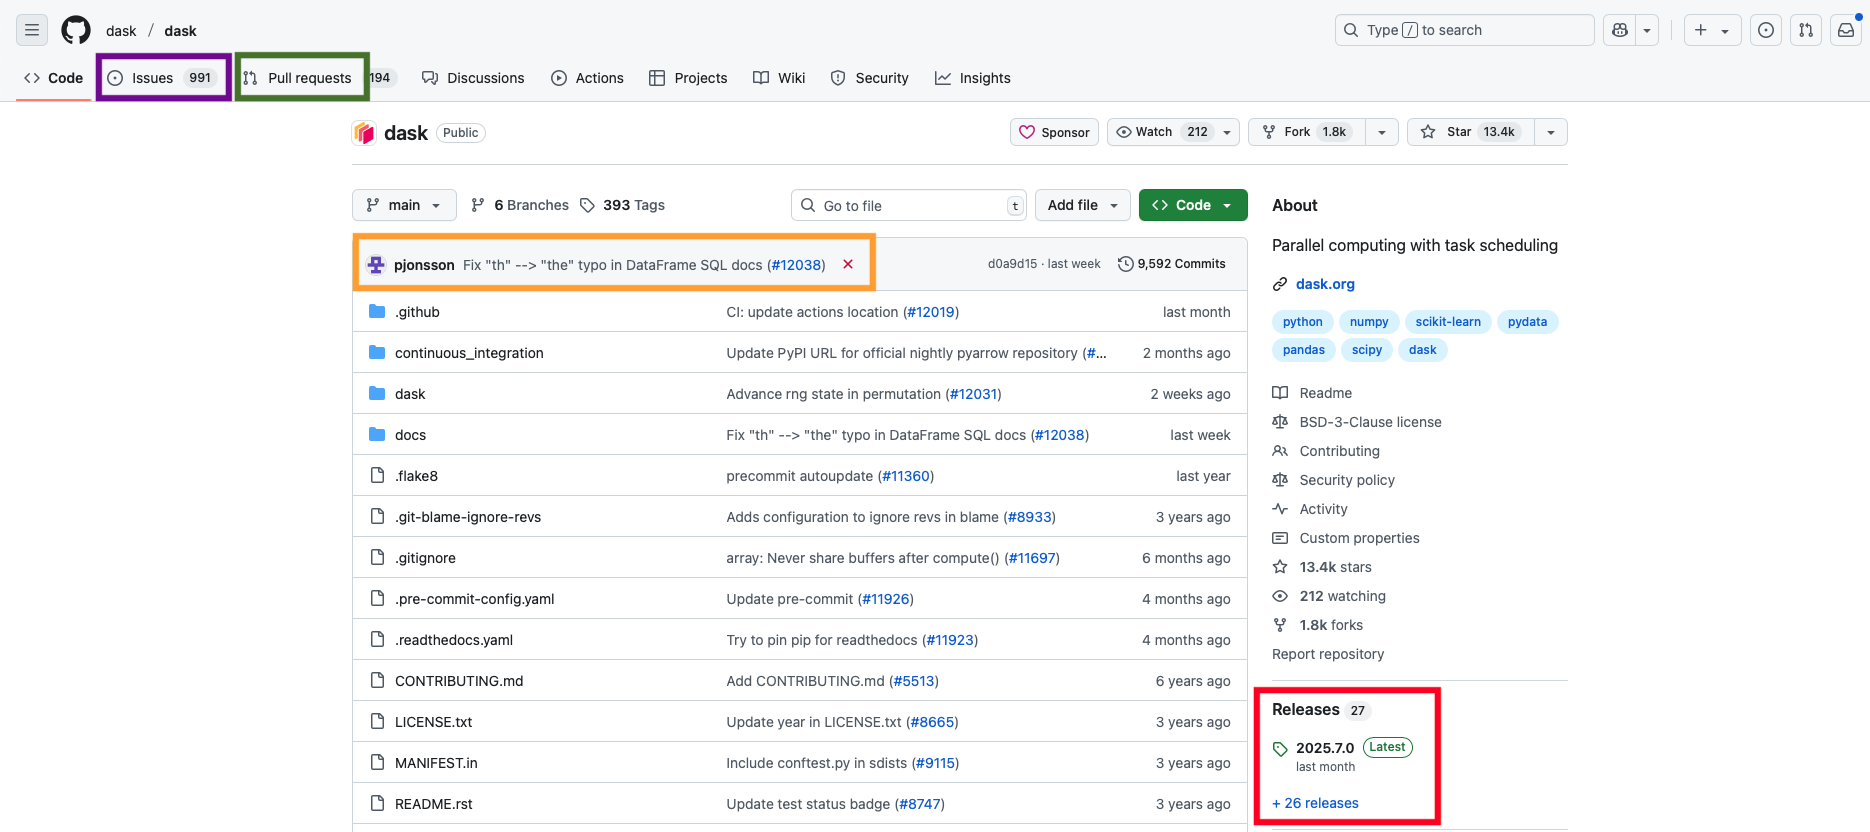
\includegraphics[width=\textwidth]{temp/dask_explainers/dask_homepage.png}
  \end{subfigure}

  \medskip

  \begin{subfigure}[b]{0.9\textwidth}
    \centering
    \caption{Example issue thread}\label{fig:dask-issue}
    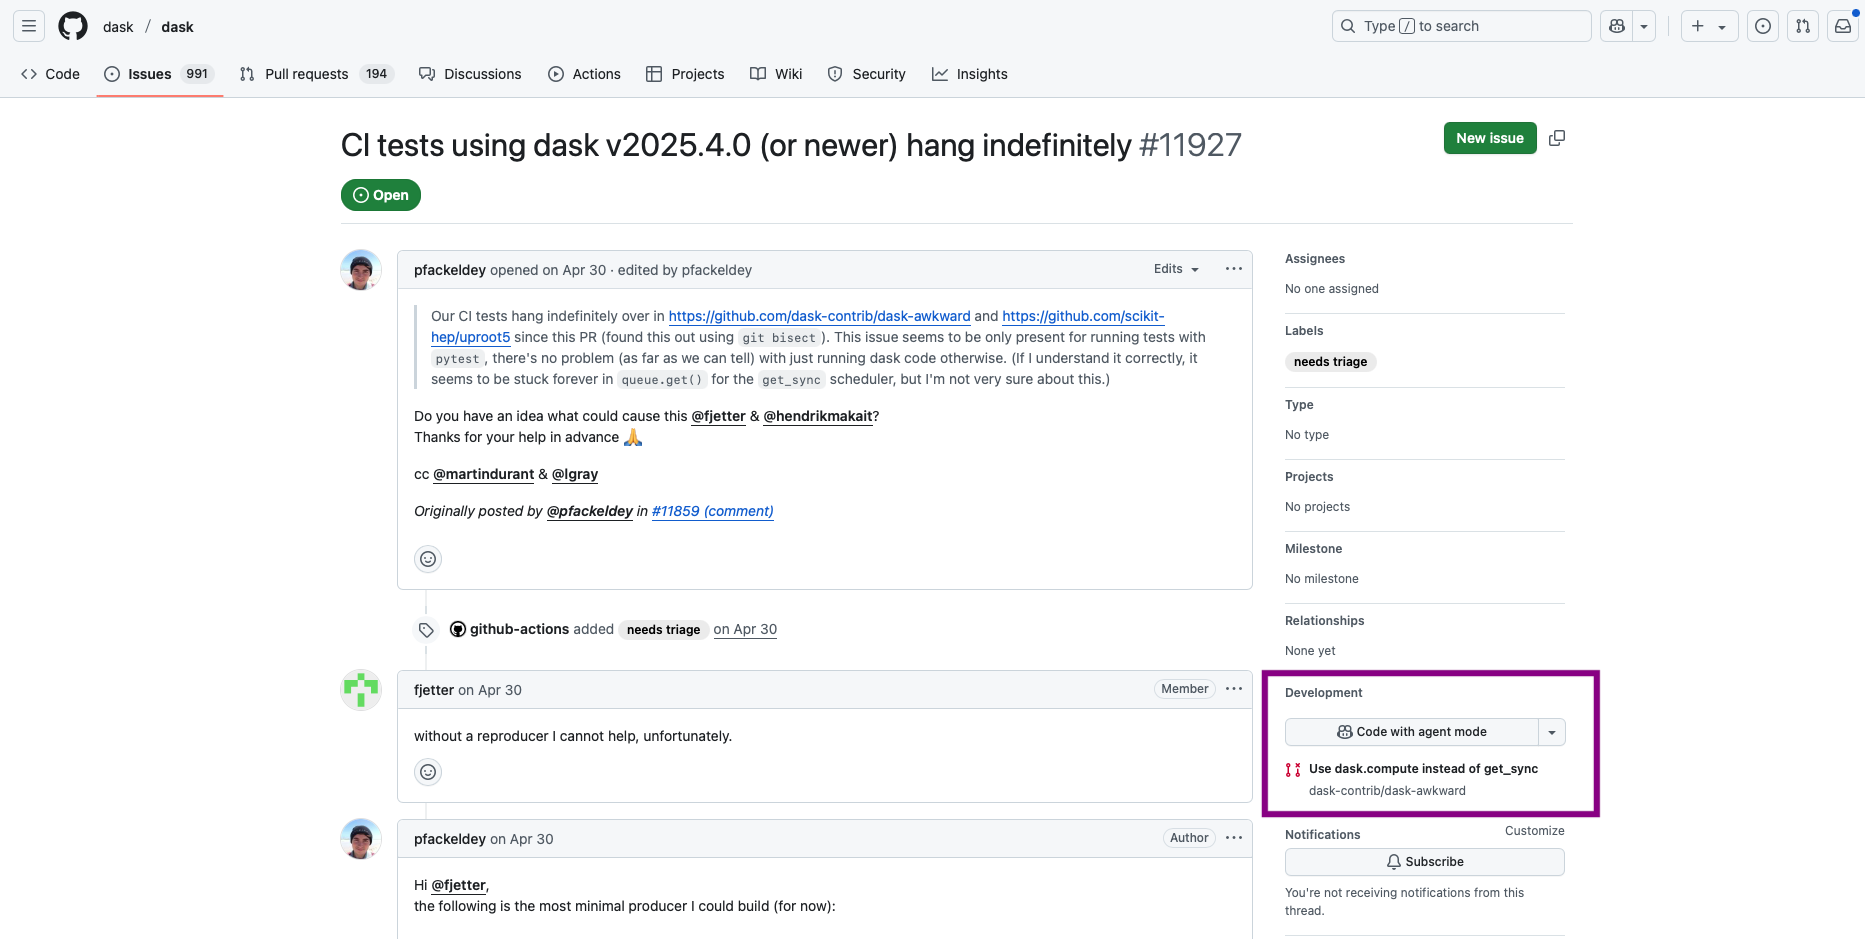
\includegraphics[width=\textwidth]{temp/dask_explainers/issue_thread.png}
  \end{subfigure}

    \bigskip
  \vspace{1ex}
  \centering
  \begin{minipage}{0.9\textwidth}
    \textbf{Figure notes:} 
    Panel~\subref{fig:dask-home} shows the \texttt{dask/dask} homepage (captured Aug 10, 12:21 PM EST).  
    The purple box links to unresolved issues (count shown); the green box links to open pull requests (count shown);  
    the orange box marks the most recent commit and its author; the red box highlights the latest release details. 
    Panel~\subref{fig:dask-issue} shows an issue thread, with the red box indicating the linked pull request. The issue was opened by user \textbf{pfackeldey} on April 30th, 2025 and received a response by \textbf{fjetter} that same day. 
  \end{minipage}

  \todo[inline]{Move to source/raw, improve title of figure}

\end{figure}
\pagebreak
\begin{figure}[ht]

    \caption{Descriptive statistics of key project metrics} \label{fig:summary-stats}
  
  \centering
  \medskip

  % Panel A
\begin{subfigure}[b]{0.9\textwidth}
  \centering
  \footnotesize
  \caption{Project summary statistics}
  \label{fig:project-summary-stats}
  \begin{tabular}{@{}l r *{5}{r}@{}}
    \toprule
    Metric                        & Mean   & \multicolumn{5}{c}{Percentiles} \\
    \cmidrule(lr){3-7}
                                  &        & 10th   & 25th   & 50th   & 75th   & 90th   \\
    \midrule
    Contributors                   & 106.72 & 9      & 20     & 49     & 120    & 239    \\
    Problems                       & 204.99 & 11     & 35     & 89     & 257    & 562    \\
    Unlinked issues                & 110.61 & 4      & 15     & 44     & 146    & 292    \\
    Unlinked pull requests         & 73.77  & 3      & 10     & 28     & 80     & 170    \\
    Linked issue–pull request pairs & 20.61  & 0      & 1      & 5      & 20     & 53     \\
    Discussions per problem        & 4.03   & 2      & 2.76   & 3.67   & 4.82   & 6.46   \\
    Contributors per problem       & 1.95   & 1.45   & 1.68   & 1.96   & 2.19   & 2.45   \\
    Time periods per project       & 13.86  & 8      & 10     & 15     & 18     & 18     \\
    \bottomrule
  \end{tabular}
\end{subfigure}

  \bigskip

  % Panel B
  \begin{subfigure}[b]{0.9\textwidth}
\caption{Contributor counts by filtering stage} \label{fig:departed-summary-stats}
    \centering
    \small
    \begin{tabular}{@{}p{0.65\textwidth} r@{}}
      \toprule
      Filter & \multicolumn{1}{c}{Contributors Remaining} \\
      \midrule
      All contributors                                    & 1,076,901 \\
      $\ge 3$ consecutive periods above 75th pct.\ commits &   13,773   \\
      Made 0 commits after departure                      &    7,646   \\
      In projects with only one departure                 &    1,594   \\
      Excluding departures from projects abandoned ≤ 3 periods later or contributors who remained active in the project &    262   \\
      In projects with $\ge 2$ important contributors     &       92   \\
      \bottomrule
    \end{tabular}
  \end{subfigure}
    \bigskip
  % Notes and overall caption
  \vspace{1ex}
  \begin{minipage}{0.9\textwidth}
    \small
    \textbf{Table Notes:}
    Panel~\subref{fig:project-summary-stats} presents the mean and selected percentiles (10th, 25th, 50th, 75th, 90th) for key project–period metrics: number of contributors, problems, unlinked issues, unlinked pull requests, linked issue–pull request pairs, discussions per problem, and contributors per problem. All statistics are based on project–time period observations. The last row includes the mean and selected percentiles for the number of periods each project appears in. 
    Panel~\subref{fig:departed-summary-stats} shows the number of contributors remaining after each filtering step.
  \end{minipage}


\end{figure}
\pagebreak

\begin{figure}[htbp]
    \centering
    \begin{minipage}[b]{0.49\textwidth}
        \centering
        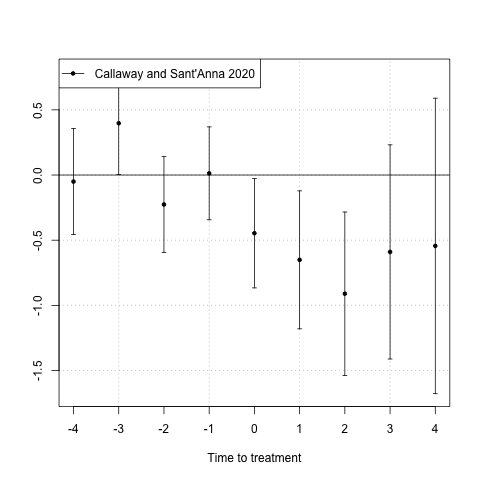
\includegraphics[width=\textwidth]{temp/output/prs_opened_norm.png}
        \subcaption{All projects}
        \label{fig:all_prs_opened}
    \end{minipage}
    \hfill
    \begin{minipage}[b]{0.49\textwidth}
        \centering
        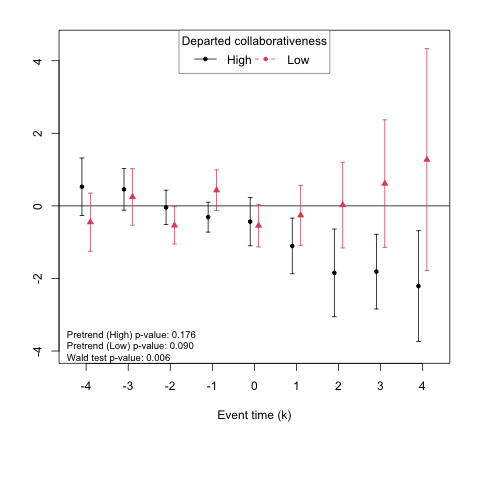
\includegraphics[width=\textwidth]{temp/output/collab/prs_opened_collab_cs_norm.png}
        \subcaption{By departed contributor collaborativeness}
        \label{fig:all_prs_opened_collab}
    \end{minipage}
    \caption{Impact of Key Contributor Departures on Project Outcomes}
    \label{fig:prs_opened}
\end{figure}

\begin{figure}[htbp]
    \caption{Impact of Departures on Others}
    \label{fig:prs_opened_other_contr}
    \centering
    \begin{minipage}[b]{0.49\textwidth}
        \centering
        \subcaption{Joined pre-departure} \label{fig:predep_prs_opened_collab}
        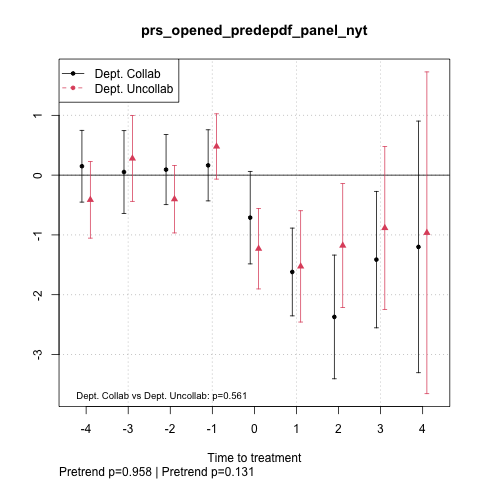
\includegraphics[width=\textwidth]{temp/output/collab/cs_norm_prs_opened_predep.png}
    \end{minipage}
    \hfill
    \begin{minipage}[b]{0.49\textwidth}
        \centering
        \subcaption{All but departed} \label{fig:nondep_prs_opened_collab}
        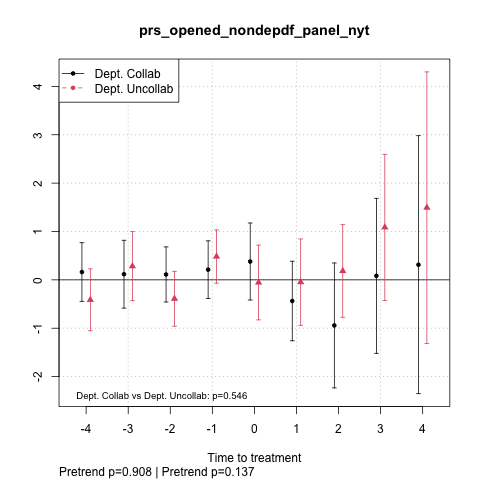
\includegraphics[width=\textwidth]{temp/output/collab/cs_norm_prs_opened_nondep.png}
    \end{minipage}

  \vspace{1ex}
  \centering
  \begin{minipage}{1\textwidth}
    \textbf{Figure notes:} 
    Following Callaway and Sant’Anna (2021), I estimate event-study coefficients accompanied by 95\% simultaneous confidence bands. For each plot with event study estimates from two subsamples, I report three Wald-test p-values: one for the pretrend test in the first subsample, one for the pretrend test in the second subsample (both from Equation \ref{eq:wald_test_pretrends} in Section \ref{sec:main_method}), and one for the difference in treatment effects across subsamples (Equation \ref{eq:wald_test} in Section \ref{sec:att_subset}). Panel~\subref{fig:predep_prs_opened_collab} depicts event study estimates from replacing the standardized outcome’s total pull request count with that of the \textbf{Pre-departure} member subset (Section~\ref{sec:contr_subset}). Panel~\subref{fig:all_prs_opened_collab} depicts event study estimates from replacing the standardized outcome’s total pull request count with that of the \textbf{Non-departure} member subset (Section~\ref{sec:contr_subset}). Both panels depict separate event study estimates for organizations with high and low departed collaborativeness. 
  \end{minipage}
\end{figure}

\begin{figure}[htbp]   
    \caption{Impact of Departed Importance on Organizational Outcomes} \label{fig:prs_opened_more_imp}
    \centering
    \begin{minipage}[b]{0.49\textwidth}
        \centering
        \subcaption{By problem involvement}    \label{fig:prs_opened_involved}
        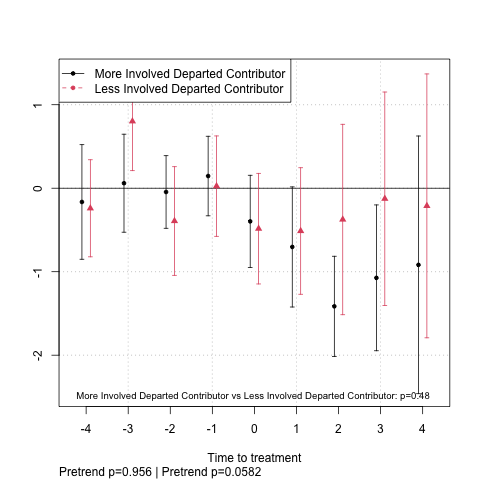
\includegraphics[width=\textwidth]{temp/output/collab/prs_opened_involved_cs_norm.png}
    \end{minipage}
    \begin{minipage}[b]{0.49\textwidth}
        \centering
        \subcaption{By PR opening involvement}    \label{fig:prs_opened_pr_involved}
        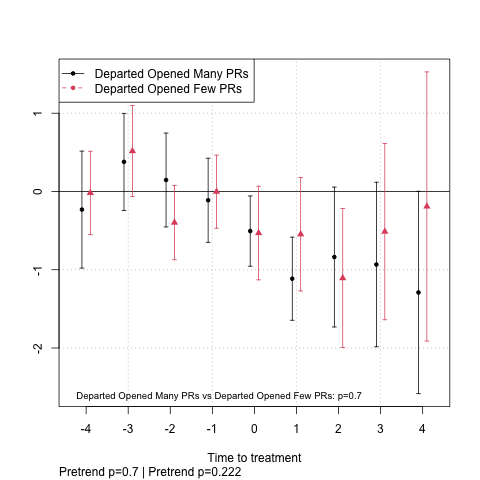
\includegraphics[width=\textwidth]{temp/output/collab/prs_opened_departed_opened_cs_norm.png}
    \end{minipage}
    \begin{minipage}[b]{0.49\textwidth}
        \centering
        \subcaption{More involved}    \label{fig:prs_opened_more_involved}
        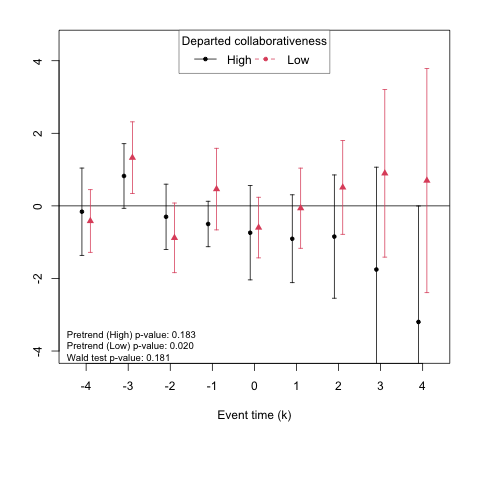
\includegraphics[width=\textwidth]{temp/output/collab_imp/inv0_cs_norm_prs_opened.png}
    \end{minipage}
    \begin{minipage}[b]{0.49\textwidth}
        \centering
        \subcaption{Less involved }    \label{fig:prs_opened_less_involved}
        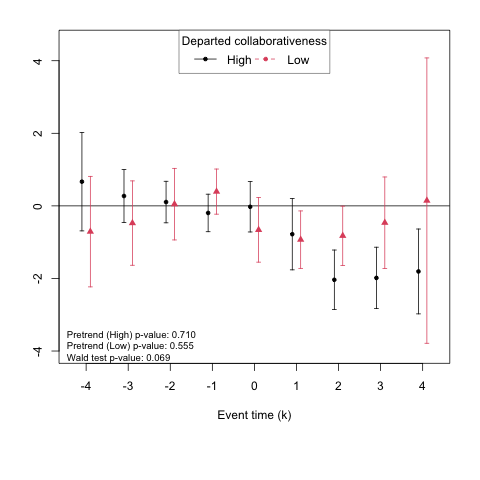
\includegraphics[width=\textwidth]{temp/output/collab_imp/inv1_cs_norm_prs_opened.png}
    \end{minipage}

  \begin{minipage}{1\textwidth}
    \textbf{Figure notes:} 
    Following Callaway and Sant’Anna (2021), I estimate event-study coefficients accompanied by 95\% simultaneous confidence bands. For each plot with event study estimates from two subsamples, I report three Wald-test p-values: one for the pretrend test in the first subsample, one for the pretrend test in the second subsample (both from Equation \ref{eq:wald_test_pretrends} in Section \ref{sec:main_method}), and one for the difference in treatment effects across subsamples (Equation \ref{eq:wald_test} in Section \ref{sec:att_subset}).  Panel~\subref{fig:prs_opened_involved}  subsets organizations by \textbf{departed member involvement}, as defined in Section~\ref{sec:org_level_subset}. Panel~\subref{fig:prs_opened_pr_involved}  subsets organizations by \textbf{departed member pull request involvement}, as defined in Section~\ref{sec:org_level_subset}. Panel~\subref{fig:prs_opened_more_involved} and Panel~\subref{fig:prs_opened_less_involved} condition on organizations where the departed was more and less involved by \textbf{departed member pull request involvement}, respectively and both subset by departed contributor collaborativeness
  \end{minipage}

\end{figure}

\begin{figure}[htbp]
    \caption{Impact of Departures on Others by Extensive Margin Communication History}
    \label{fig:prs_opened_comm_ext_marg}
    \centering
        \begin{minipage}[b]{0.49\textwidth}
        \centering
        \subcaption{Highly collaborative} \label{fig:predep_prs_opened_high_collab_comm_ext_marg}
        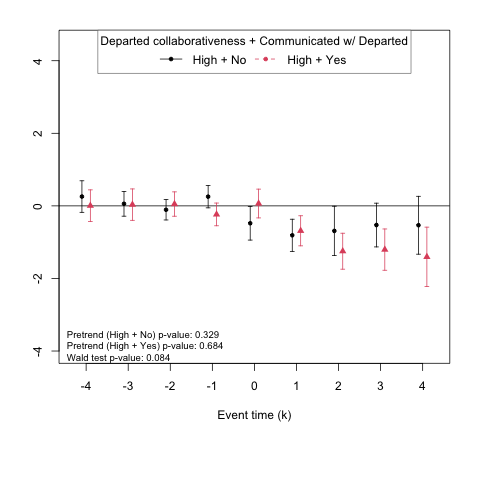
\includegraphics[width=\textwidth]{temp/output/collab/cs_norm_prs_opened_dept_never_comm_predep_High.png}
    \end{minipage}
    \hfill
    \label{fig:prs_opened_comm_ext_marg_low}
    \centering
        \begin{minipage}[b]{0.49\textwidth}
        \centering
        \subcaption{Less collaborative } \label{fig:predep_prs_opened_low_collab_comm_ext_marg}
        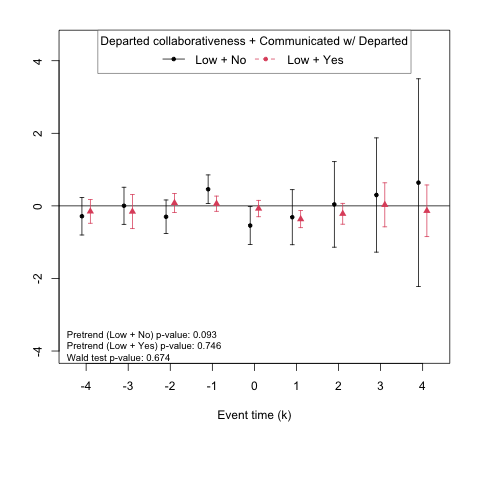
\includegraphics[width=\textwidth]{temp/output/collab/cs_norm_prs_opened_dept_never_comm_predep_Low.png}
    \end{minipage}
    
  \begin{minipage}{1\textwidth}
    \textbf{Figure notes:} 
    Following Callaway and Sant’Anna (2021), I estimate event-study coefficients accompanied by 95\% simultaneous confidence bands. For each plot with event study estimates from two subsamples, I report three Wald-test p-values: one for the pretrend test in the first subsample, one for the pretrend test in the second subsample (both from Equation \ref{eq:wald_test_pretrends} in Section \ref{sec:main_method}), and one for the difference in treatment effects across subsamples (Equation \ref{eq:wald_test} in Section \ref{sec:att_subset}). 
    Panel~\subref{fig:predep_prs_opened_high_collab_comm_ext_marg} replaces the standardized outcome’s total pull request count with that of two different member subsets: members who had ever \textbf{communicated with the departed} and members who had \textbf{never communicated with the departed} prior to estimation (as defined in Section~\ref{sec:contr_subset}) and conditions on organizations with highly collaborative departed members.
    Panel~\subref{fig:predep_prs_opened_low_collab_comm_ext_marg} is the analog of Panel~\subref{fig:predep_prs_opened_high_collab_comm_ext_marg} for less collaborative departed members.  
  \end{minipage}
  

\end{figure}

\begin{figure}
    \caption{Impact of Departures on Others by Communication History and Involvement}
    \label{fig:prs_opened_comm_ext_marg_inv}
    \centering
    \begin{minipage}[b]{0.48\textwidth}
        \centering
        \subcaption{Less involved, highly collaborative} \label{fig:predep_prs_opened_high_collab_comm_ext_marg_inv0}
        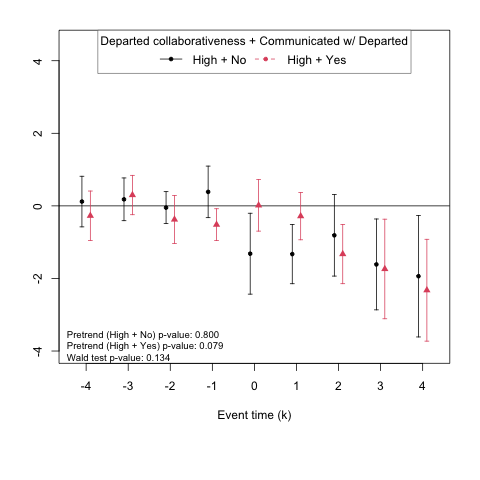
\includegraphics[width=\textwidth]{temp/output/collab_imp/inv0_cs_norm_prs_opened_dept_never_comm_predep_High.png}
    \end{minipage}
    \hfill
    \begin{minipage}[b]{0.48\textwidth}
        \centering
        \subcaption{Less involved and collaborative} \label{fig:predep_prs_opened_low_collab_comm_ext_marg_inv0}
        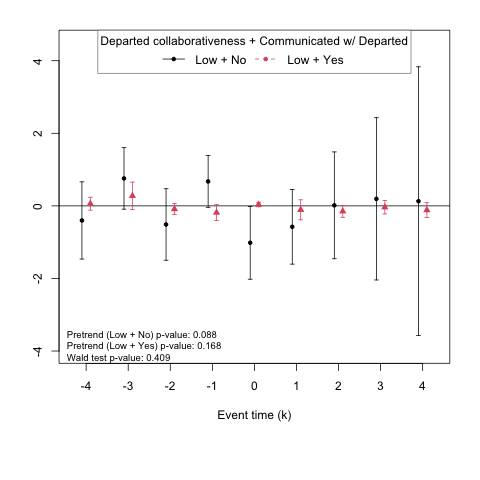
\includegraphics[width=\textwidth]{temp/output/collab_imp/inv0_cs_norm_prs_opened_dept_never_comm_predep_Low.png}
    \end{minipage}
    \begin{minipage}[b]{0.48\textwidth}
        \centering
        \subcaption{Highly involved and collaborative} \label{fig:predep_prs_opened_high_collab_comm_ext_marg_inv1}
        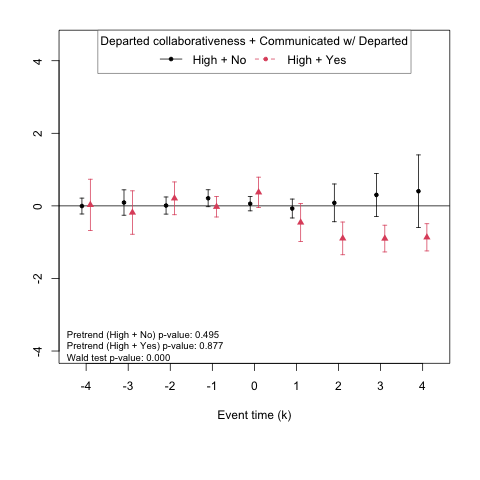
\includegraphics[width=\textwidth]{temp/output/collab_imp/inv1_cs_norm_prs_opened_dept_never_comm_predep_High.png}
    \end{minipage}
    \hfill
    \begin{minipage}[b]{0.48\textwidth}
        \centering
        \subcaption{Highly involved, less collaborative} \label{fig:predep_prs_opened_low_collab_comm_ext_marg_inv1}
        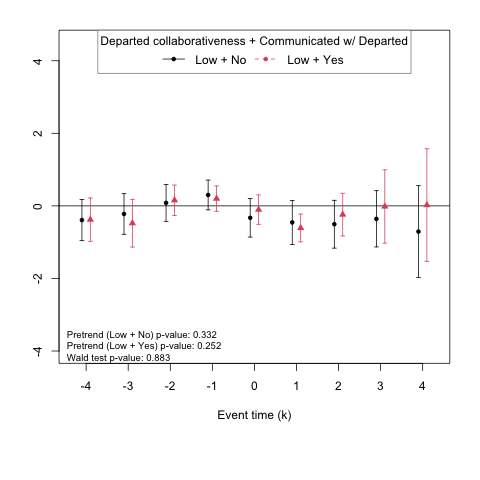
\includegraphics[width=\textwidth]{temp/output/collab_imp/inv1_cs_norm_prs_opened_dept_never_comm_predep_Low.png}
    \end{minipage}

  \begin{minipage}{1\textwidth}
    \textbf{Figure notes:} 
    Following Callaway and Sant’Anna (2021), I estimate event-study coefficients accompanied by 95\% simultaneous confidence bands. For each plot with event study estimates from two subsamples, I report three Wald-test p-values: one for the pretrend test in the first subsample, one for the pretrend test in the second subsample (both from Equation \ref{eq:wald_test_pretrends} in Section \ref{sec:main_method}), and one for the difference in treatment effects across subsamples (Equation \ref{eq:wald_test} in Section \ref{sec:att_subset}). Panel~\subref{fig:predep_prs_opened_high_collab_comm_ext_marg_inv0} is the analog of Panel~\subref{fig:predep_prs_opened_high_collab_comm_ext_marg} from Figure~\ref{fig:prs_opened_comm_ext_marg}, but additionally conditions on organizations with highly collaborative departed members who were less involved. Panel~\subref{fig:predep_prs_opened_low_collab_comm_ext_marg_inv0}, Panel~\subref{fig:predep_prs_opened_high_collab_comm_ext_marg_inv1} and Panel~\subref{fig:predep_prs_opened_low_collab_comm_ext_marg_inv1} are the analog of Panel~\subref{fig:predep_prs_opened_high_collab_comm_ext_marg_inv0} for organizations with less collaborative and less involved departed members, highly collaborative and involved departed member, and less collaborative and highly involved departed members, respectively. 
\end{minipage}
  

\end{figure}

\begin{figure}[htbp]
    \caption{Subsetting by contributor communication intensity}
    \label{fig}
    \centering
    \begin{minipage}[b]{0.49\textwidth}
        \centering
        \subcaption{Communication (lifetime)} \label{fig}
        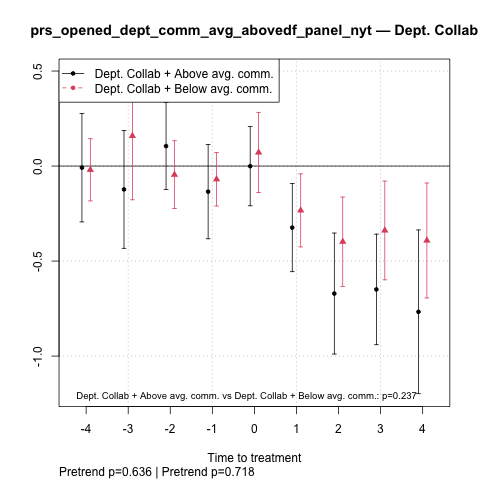
\includegraphics[width=\textwidth]{temp/output/collab/cs_norm_prs_opened_dept_comm_avg_above_Dept.Collab.png}
    \end{minipage}
    \hfill
    \begin{minipage}[b]{0.49\textwidth}
        \centering
        \subcaption{Communication per Problem}\label{fig}
        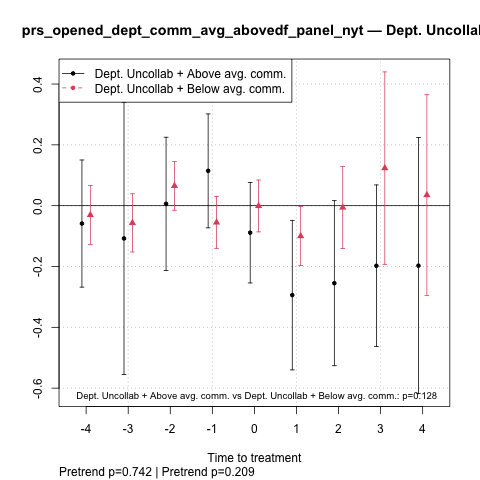
\includegraphics[width=\textwidth]{temp/output/collab/cs_norm_prs_opened_dept_comm_avg_above_Dept.Uncollab.png}
    \end{minipage}
        \begin{minipage}[b]{0.49\textwidth}
        \centering
        \subcaption{Communication (lifetime)} \label{fig}
        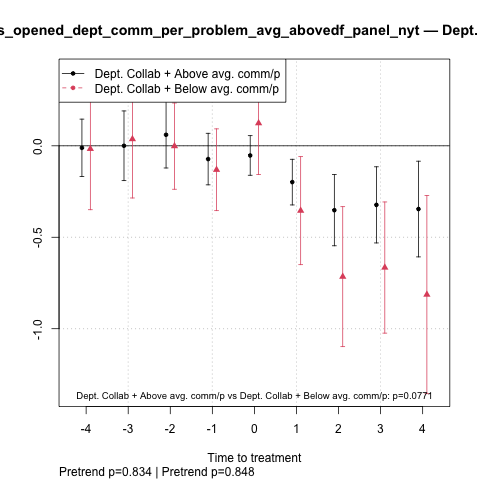
\includegraphics[width=\textwidth]{temp/output/collab/cs_norm_prs_opened_dept_comm_per_problem_avg_above_Dept.Collab.png}
    \end{minipage}
    \hfill
    \begin{minipage}[b]{0.49\textwidth}
        \centering
        \subcaption{Communication per Problem}\label{fig}
        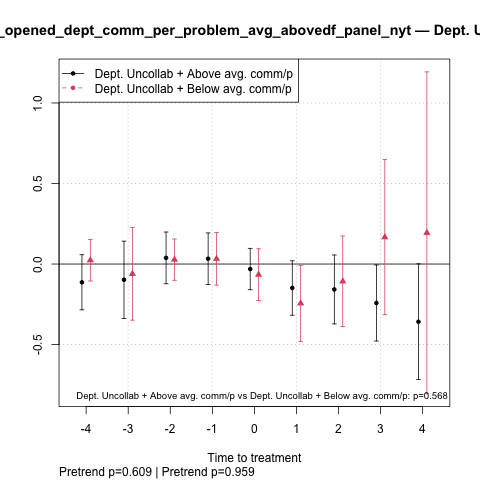
\includegraphics[width=\textwidth]{temp/output/collab/cs_norm_prs_opened_dept_comm_per_problem_avg_above_Dept.Uncollab.png}
    \end{minipage}


\todo[inline]{Graph improvements
1. Align axis for Panel a and b to -3.5 to 4.5 with ticks at every .5 (or 1)\\
2. Add figure notes describing definition of collaboration, confidence intervals (bootstrap 95 CI). \\
3. Change legend to indicate "Departed Contributor Collaborativeness" and have values be collaborative uncollaborative. \\
4. Remove grid background\\
5. Change time to treatment to "event time (k)"\\
6. Remove ugly bold label\\
7. Fine tune the plot subtitles
}

\end{figure}

\begin{figure}[htbp]
    \caption{Drivers of the Impact of Departures on Others }
    \label{fig:prs_opened_comm_int_marg_avg}
    \centering
    \begin{minipage}[b]{0.48\textwidth}
        \centering
        \subcaption{Less involved, highly collaborative} \label{fig:predep_prs_opened_high_collab_comm_inv0_rep}
        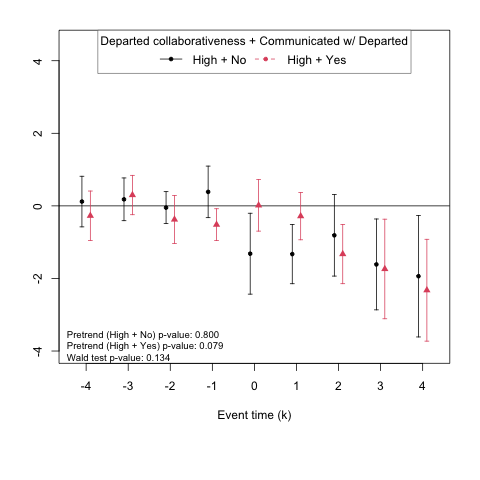
\includegraphics[width=\textwidth]{temp/output/collab_imp/inv0_cs_norm_prs_opened_dept_never_comm_predep_High.png}
    \end{minipage}
    \hfill
    \begin{minipage}[b]{0.48\textwidth}
        \centering
        \subcaption{Holding participation constant} \label{fig:predep_n_avg_prs_opened_high_collab_comm_inv0}
        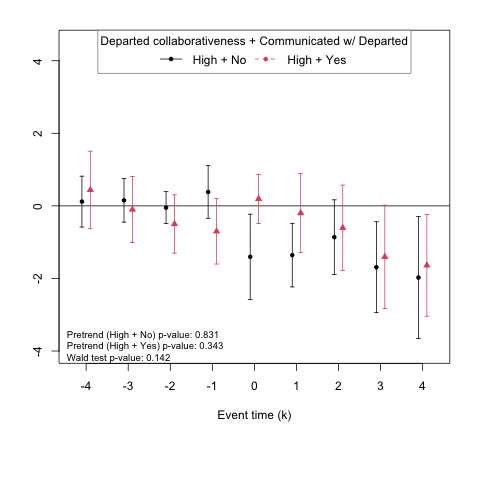
\includegraphics[width=\textwidth]{temp/output/collab_imp/inv0_cs_norm_n_avg_prs_opened_dept_never_comm_predep_High.png}
    \end{minipage}
    \begin{minipage}[b]{0.48\textwidth}
        \centering
        \subcaption{Highly involved and collaborative} \label{fig:predep_prs_opened_high_collab_comm_inv1_rep}
        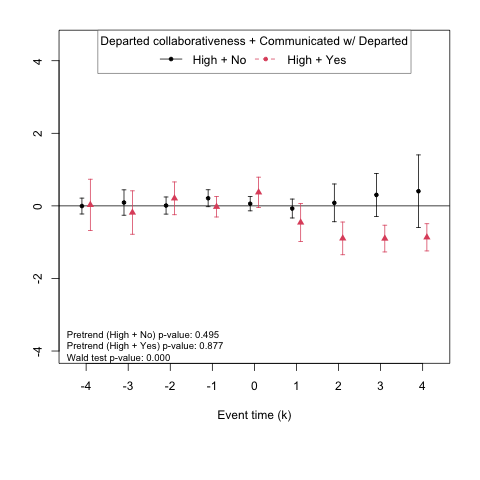
\includegraphics[width=\textwidth]{temp/output/collab_imp/inv1_cs_norm_prs_opened_dept_never_comm_predep_High.png}
    \end{minipage}
    \hfill
    \begin{minipage}[b]{0.48\textwidth}
        \centering
        \subcaption{Holding participation constant} \label{fig:predep_n_avg_prs_opened_high_collab_comm_inv1}
        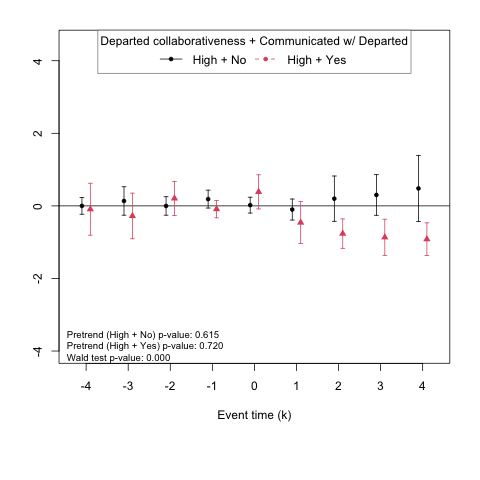
\includegraphics[width=\textwidth]{temp/output/collab_imp/inv1_cs_norm_n_avg_prs_opened_dept_never_comm_predep_High.png}
    \end{minipage}

  \begin{minipage}{\textwidth}
    \textbf{Figure notes:} 
    Following Callaway and Sant’Anna (2021), I estimate event-study coefficients accompanied by 95\% simultaneous confidence bands. For each plot with event study estimates from two subsamples, I report three Wald-test p-values: one for the pretrend test in the first subsample, one for the pretrend test in the second subsample (both from Equation \ref{eq:wald_test_pretrends} in Section \ref{sec:main_method}), and one for the difference in treatment effects across subsamples (Equation \ref{eq:wald_test} in Section \ref{sec:att_subset}). Panel~\subref{fig:predep_prs_opened_high_collab_comm_inv0_rep} is the same as Panel~\subref{fig:predep_prs_opened_high_collab_comm_ext_marg_inv0} from Figure~\ref{fig:prs_opened_comm_ext_marg_inv}. Panel~\subref{fig:predep_n_avg_prs_opened_high_collab_comm_inv0} depicts event study estimates from the counterfactual where average activity per member evolves factually based on Panel~\subref{fig:predep_prs_opened_high_collab_comm_inv0_rep} but I assume that member participation remains at the level of $k=-1$. anel~\subref{fig:predep_prs_opened_high_collab_comm_inv1_rep} and Panel~\subref{fig:predep_n_avg_prs_opened_high_collab_comm_inv1} are the analogs of  Panel~\subref{fig:predep_prs_opened_high_collab_comm_inv0_rep}  and Panel~\subref{fig:predep_prs_opened_high_collab_comm_inv0_rep}, respectively, for organizations with highly collaborative and involved departed members. 
    
  \end{minipage}
  


\end{figure}

\begin{figure}[htbp]
    \caption{Impact of Contributor Departures by Other Collaboration}
    \label{fig:prs_opened_other_fig}
    \centering
    \begin{minipage}[b]{0.48\textwidth}
        \centering
        \subcaption{By other collaboration} \label{fig:prs_opened_other}
        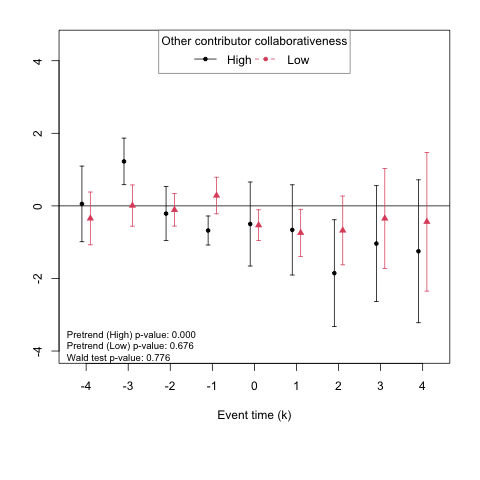
\includegraphics[width=\textwidth]{temp/output/collab/prs_opened_other_collab_cs_norm.png}
    \end{minipage}
  \begin{minipage}{\textwidth}
    \textbf{Figure notes:} 
    Following Callaway and Sant’Anna (2021), I estimate event-study coefficients accompanied by 95\% simultaneous confidence bands. For each plot with event study estimates from two subsamples, I report three Wald-test p-values: one for the pretrend test in the first subsample, one for the pretrend test in the second subsample (both from Equation \ref{eq:wald_test_pretrends} in Section \ref{sec:main_method}), and one for the difference in treatment effects across subsamples (Equation \ref{eq:wald_test} in Section \ref{sec:att_subset}). 
    Panel~\subref{fig:prs_opened_other} plots two sets of event study estimates: projects with high and low collaboration among other key contributors (as defined in Section~\ref{sec:collab_imp_contr}). In all panels, the outcome is the pull request z score, transformed using the pre-treatment mean and standard deviation.

  \end{minipage}
\end{figure}

\begin{figure}[ht]
  \centering

    \caption{Pre-departure outcome distribution}\label{fig:tradeoffs}
  \medskip
  \begin{subfigure}[b]{0.9\textwidth}
    \centering
    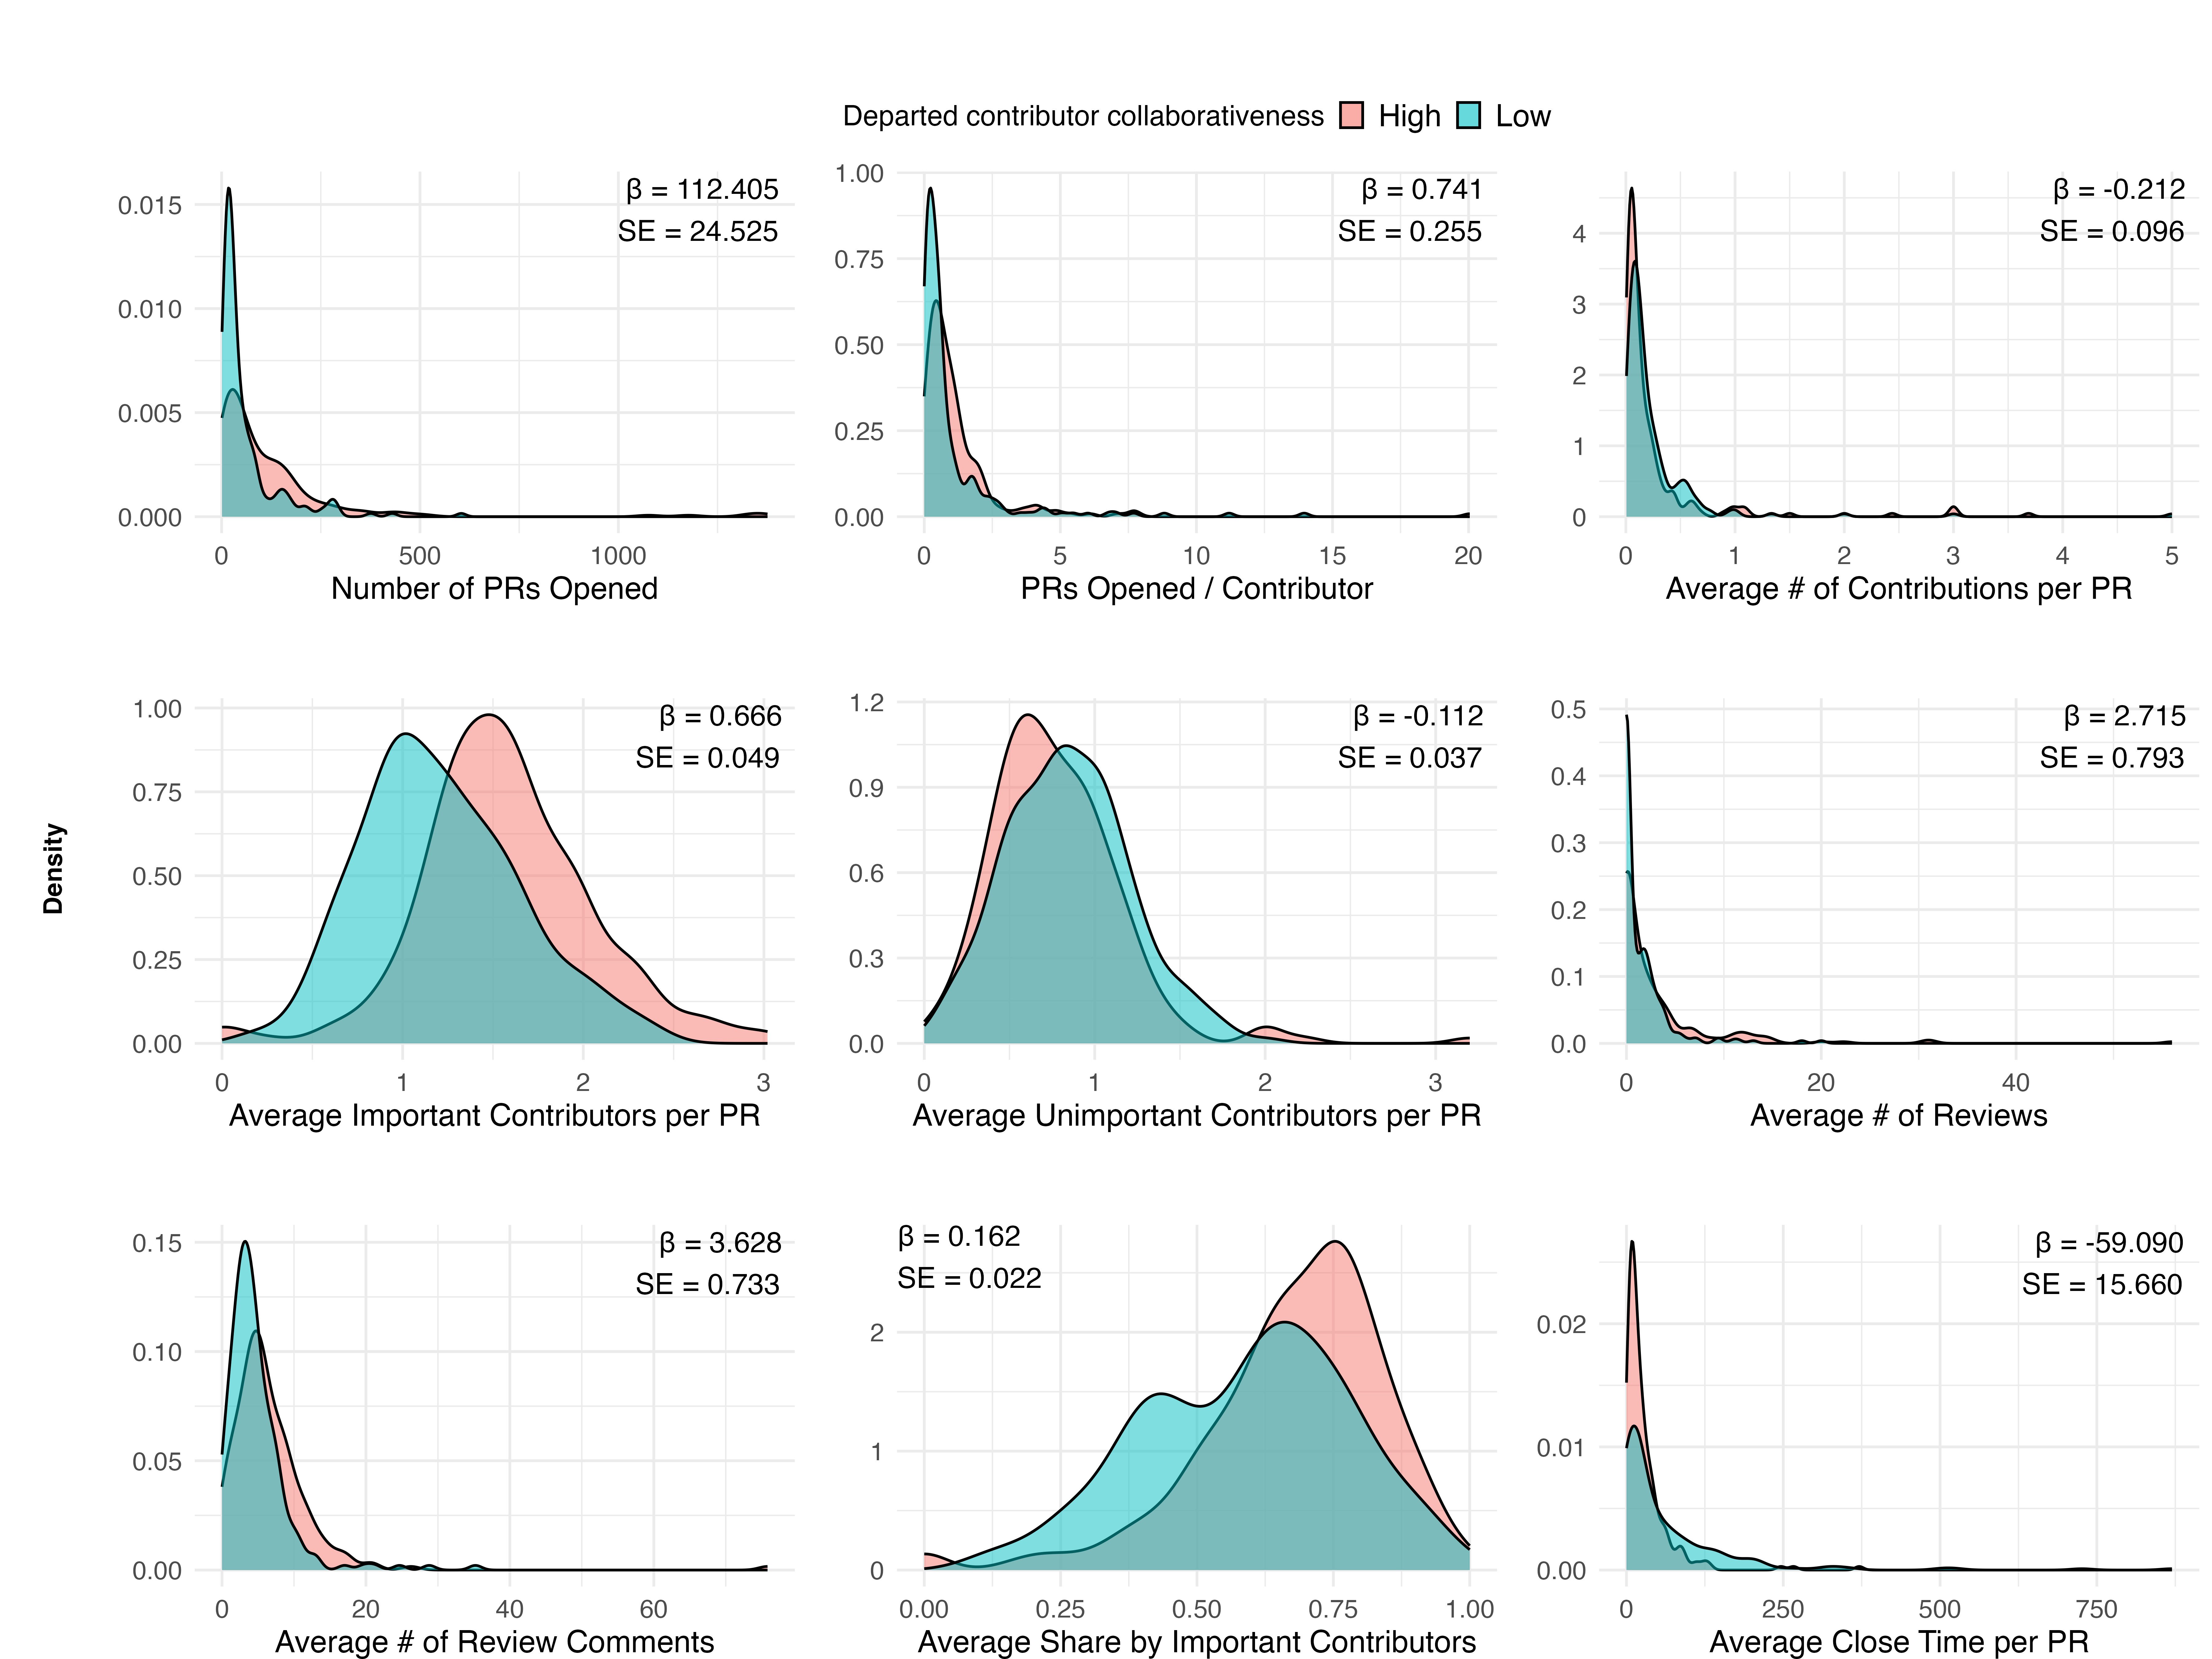
\includegraphics[width=\textwidth]{temp/output/collab_outcomes.png}
  \end{subfigure}

    \bigskip
  \vspace{1ex}
  \centering
  \begin{minipage}{0.9\textwidth}
    \textbf{Figure notes:} In each panel, I display a density plot of the labelled outcome during pre-departure periods for organizations with and without highly collaborative departed contributors. Each observation is at the organization-time period level. The statistics on the rop right for each panel are the regression coefficient and standard error for regressing the outcome on departed contributor collaborativeness (in its continuous form). 
  \end{minipage}

  \longterm[inline]{Move to source/raw, improve title of figure}

\end{figure}
\pagebreak
\begin{figure}[!htbp]
\centering
\caption{Determinants of pull request close time}
\label{fig:close_time_regression}
{\small
\begin{tabular}{lll}
\hline
& Pull request closing time &  \\ \cmidrule(lr){2-3}
& Coefficient & SE \\ \hline
Average \# of reviews & 0.561 & 0.505 \\
Average qty of discussion per PR & -24.686 & 16.208 \\
Proportion w/ no Reviews & -21.790 & 15.996 \\
Departed member collaborativeness & -23.585 & 13.572 \\
Average \# of umportant members & 9.013 & 8.826 \\
Average \# of unimportant members & -42.027 & 25.096 \\
Average share by important members & -226.375 & 66.115 \\
\hdashline
Obs & 308 & \\
Time FE & X &  \\
\hline
\end{tabular}
}
  \begin{minipage}{\textwidth}
    \small
    \textbf{Table Notes:}  Figure~\ref{fig:close_time_regression} presents the coefficients from a regression of how much time it takes to close a pull request on the average \# of reviews on a pull request, the average amount of discussion  by members per pull request, the proportion of pull requests in a organization without reviews, the continuous value of departed member collaborativeness, the average \# of important and unimportant members in an organization and the average share of discussion done by important contributors in pull requests.
    Each observation is at the organization-time period level, time fixed effects are included and standard errors are clustered at the organization level. 
  \end{minipage}

\longterm[inline]{automate}
\end{figure}



\clearpage
\onehalfspacing

\section*{Appendix (Future goals)}\label{sec:appendixa}
\subsection{Questiosn for Jesse}
\begin{enumerate}
\item Do you see an obvious place for a model. See below for old model notes
\iffalse
Model of hierarchy incorporates cooperation and communication as key features of the hierarchy that affect downstream organization outcomes. However, I take these for granted and irl, communication and cooperation can't be taken for granted
\begin{enumerate}
\item Extent of communication 
\item Degree of cooperation, overlap (clustering)
\end{enumerate}

Existing theory tells us how organizations adapt their organizational structure and strategy in response to external shocks. However, it doesn't tell us how that adaption depends on existing organizational structure. One example: communication is an integral part of how an organization solves problems, but I don't model how it occurs. Moreover, communication itself also has pros and cons - does it have a positive effect by sharing knowledge or negative effect by creating reliance and thus inhibiting learning?

% See https://www.sciencedirect.com/science/article/abs/pii/S0268401217310095 for a survey of current work
- Doesn't try to separate relationship between structure and departures
- Does not consider the complementarity of organizational structure 
- Research on impact of organizational structures only provides suggestive evidence on the mechanism by which organizational structures have impacts. 
- The focus of research has been on codebase related outcomes or "organization survival" as opposed to more relevant outcomes such as usage. 
\fi 
\end{enumerate}

\subsection{Improvements}
\begin{enumerate}
\item Can I implement the bin scatter with downstream outcomes such as downloads, releases and software quality. Can I also explore other OSS activities such as discussions, forks
\item Does teamwork lead to increased specialization or exposure to a broader range of tasks?
\item Can I implement random forest that helps with 1) discovering what mitigates departure impact, 2) Analyzing heteorgeneity in treatment effects more smoothly and 3) what differentiates collaborative and uncollaborative organizations
\item Can I show that I'm actually only getting "one" departure by showing that organizations are close to the start of their lifetime? 
\item Try to justify the plausibility of collaboration more by showing that organizations are observably similar to organizations with uncollaborative departed members. Example factors include organization age at departure time, Forks, stars, departure date, \textbf{think of other things as well}
\end{enumerate}


\begin{itemize}
\item Appendix: How I map PyPi organizations to github repositories
\item Appendix: How I match repo names to repo ids in cases where identity changes
\item Appendix: How are commits measured and deal with the fact that push and PR commits can be overlapping? 
\item Appendix: Robustness to 3 month measurements (if necessary)
\end{itemize}
\subsubsection{Defining the set of problems (the linking process)}
\begin{enumerate}
\item First construct a mapping between issues + PRs. This helps create a dataset of "problems" that organizations address
\begin{itemize}
\item Three problem types: unlinked issues, unlinked PRs, linked
\item Construct linkage using the following criteria
\begin{enumerate}
\item Use the provided link.
\item For each remaining unlinked issue/PR, find a counterpart that mutually references it and choose the closest number.
\item If no mutual reference exists, find any one-way reference and choose the closest number
\end{enumerate}
\end{itemize}
\item Only keep organizations that have at least two important members in all pre-treatment periods (henceforth known as pre periods)
\end{enumerate}
\subsection{If this comes up, define other outcomes}


\begin{enumerate}
\item Measurement of downstream outcomes - the deifne the ones that I end up using. 
\item Describe software releases, the various types and measurement
\item Define software quality (security measure, not user experience based)
\item Downloads
\end{enumerate}

\todo[inline]{Should I characterize the intensive vs. extensive margin?}
$\bar Y_{k}^{!0} $ is average outcome among only individuals whose individual outcome exceeded 0 in period $k$. Let $p_k^{!0}$ be the proportion of individuals in period $k$ whose individual outcome exceeds 0. 
\begin{align*}
\mathbb{E}\!\left[\frac{(\bar Y_k - \bar Y_{-1}) }{\sigma_Y} \Big| T=1\right] &= \mathbb{E}\!\left[\frac{ \bar Y_{k}^{!0}p_k^{!0} - \bar Y_{-1}^{!0} p_{-1}^{!0} }{\sigma_Y} \Big| T=1\right] \\
&=\mathbb{E}\!\left[\frac{ \barY_{k}^{!0}p_k^{!0} - \barY_{k}^{!0} p_{-1}^{!0} +\bar Y_{k}^{!0}p_{-1}^{!0}-\bar Y_{-1}^{!0}p_{-1}^{!0} }{\sigma_Y} \Big| T=1\right] \\
&=\mathbb{E}\!\left[\frac{ \barY_{k}^{!0} \left(p_k^{!0} -p_{-1}^{!0}\right) +\left( \barY_{k}^{!0}- \bar Y_{-1}^{!0} \right)p_{-1}^{!0}}{\sigma_Y} \Big| T=1\right] 
\end{align*}

\todo[inline]{Estimate, ideally it's mostly intensive not extensive margin}

\subsection{Aspirational To Dos for data section }
\begin{enumerate}
\item Read this\href{https://pubs.aeaweb.org/doi/pdfplus/10.1257/jep.36.3.211}{paper} in order to understand how to motivate the paper using descriptive statistics
\item Provide insight into what a organization is like, such as
\begin{itemize}
\item What are churn rates like among both hierarchies?
\item Provide estimates of data coverage at a organization level 
\end{itemize}
\item Add reference to showing that results are not sensitive to changes in parameters/if they are, justify why mine is reasonable 
\end{enumerate}

\todo[inline]{\href{https://www.jonathandroth.com/assets/files/roth_pretrends_testing.pdf}{Check Roth for pretrends testing}}
\todo[inline]{Rule out the easy confounders/explanations first before dividing into more interesting explanations}
What I'm hoping to establish next is whether/the degree to which the decline in PRs is mechanical

\textbf{Can I turn these into robustness checks?}
\begin{enumerate}
\item Am I confounding the effect of how collaborative the departed member is with how important/involved the departed member is? 
\todo[inline]{Explain that because the denominator on departed member involvement is the \# of questions the departed is involved in, there's no mechanical relationship between departed member involvement and collaboration}
\todo[inline]{Examine what happens when I split by departed member importance. I can do this by calculating departed involvement as the proportion of problems they're involved in, and comparing event study results for the more/less involved bins x collaboration. I should also examine how things vary by more/less involved bins. I expect there to be a difference based off the more/less involved bins - I don't know what I will see when I interact collaboration with the results. }
\textcolor{blue}{Note: calculations done, called "departed\_involved\_2bin"}
\item How does collaborative score vary by 
\begin{enumerate}
\item important member count \textcolor{blue}{"key\_member\_count\_2bin"}
\item Total member count \textcolor{blue}{"total\_member\_count\_2bin"}
\item Problem count \textcolor{blue}{"problem\_count\_2bin"}
\end{enumerate}
and how do each of the factors above interact with collaborative score in determining the outcome? For the last two consider how size is related to the proportion/count difference. 
\todo[inline]{Execute the task above. Definitions should be straightforward}
\item What is the effect of collaboration among other members (No effect). Might the presence of prior collaboration among other members have an effect depending on how collaborative the departed member was? 
\todo[inline]{Describe in more detail results for other collaboration}
\todo[inline]{Execute the task above. One hypothesis is that other collaboration is only helpful when the departed member was collaborative and task allocation is required. This is because other departed members now need to reallocate what tasks they are working on to account for the departed's loss, but this reallocation only happens if there's collaboration with the deprated $\iff $ responsibiltiies can easily be reallocated}
\item Departed members can affect whether PRs are opened in two ways: By opening PRs themselves/authoring the majority of the commits involved in the PR, or by contributing to discussion that leads to PRs being opened. Can I identify how active departed members are in each and see
\begin{enumerate}
\item Whether the discussion mechanism has any effect on post-departure outcomes
\item How both factors interact with collaboration (Expect collaboration to interact with discussion in more interesting ways)
\end{enumerate}
\todo[inline]{Execute the above. 1) Does the effect of departed involvement change when I also vary by PR opening intensity (test 2 variations of opening PRs: one that excludes non-opening/commit involvement in PRS and one that does), 2) How does collaboration interact with PR opening intensity to affect outcomes, 3) What's the best way to loop departed involvement in as well - answer will be easier after I know 1}
\textcolor{blue}{Note: Calculated prop of PRs opened/authored by departed, out of all the author is involved in. Note that the denominator is all PRs implemented by the departed not all PRs implemented by the organization. If I had the denominator be total problems, I wouldn't be able to differentiate, holding departed involvement constant, organizations with high/low departed involvement because then the lower bound of departed PR opening would be mechanically increasing in departed PR involvement}
\textbf{complicated}


\item Mass departures in collaborative organizations, is there a systematic proximity to release in either

\item There's a persistent (and a decrease) in PRs opened over time, so it's not just that organizations have been abandoned. What's driving this? Are people able to somewhat wrap up problems that the departed was involved in?
\item \textbf{What is their role as a collaborator?}

\end{enumerate}

\textbf{Robustness}
\begin{enumerate}
\item What do development related characteristics look like prior to departure? I'm trying to see if I can provide quantitative evidence of "no anticipation" in that behavior across a wide range of measures is unchanged
\end{enumerate}

\todo[inline]{Other thought (NEED TO THINK ABOUT HOW THIS RELATES TO PAPER THEME): Are these problems still subject to the same level of review (unchanged quantity of pr review comments per PR) post-departure?}

\textbf{Other ways of splitting the data}
\begin{enumerate}
\item How does the effect of fast vs. slow communication affect the effect of collaboration
\end{enumerate}
\textbf{Other outcomes to consider}
\begin{itemize}
\item Are they linking issues to PRs at higher rates or closing issues at lower rates?
\item D\textbf{oes their language evolve to be more similar to the departed's?}
\item Do they solve problems that are outside of their realm (using issue tags or language similarity)?
\end{itemize}

\end{document}